% Options for packages loaded elsewhere
\PassOptionsToPackage{unicode}{hyperref}
\PassOptionsToPackage{hyphens}{url}
%
\documentclass[
]{book}
\usepackage{amsmath,amssymb}
\usepackage{lmodern}
\usepackage{iftex}
\ifPDFTeX
  \usepackage[T1]{fontenc}
  \usepackage[utf8]{inputenc}
  \usepackage{textcomp} % provide euro and other symbols
\else % if luatex or xetex
  \usepackage{unicode-math}
  \defaultfontfeatures{Scale=MatchLowercase}
  \defaultfontfeatures[\rmfamily]{Ligatures=TeX,Scale=1}
\fi
% Use upquote if available, for straight quotes in verbatim environments
\IfFileExists{upquote.sty}{\usepackage{upquote}}{}
\IfFileExists{microtype.sty}{% use microtype if available
  \usepackage[]{microtype}
  \UseMicrotypeSet[protrusion]{basicmath} % disable protrusion for tt fonts
}{}
\makeatletter
\@ifundefined{KOMAClassName}{% if non-KOMA class
  \IfFileExists{parskip.sty}{%
    \usepackage{parskip}
  }{% else
    \setlength{\parindent}{0pt}
    \setlength{\parskip}{6pt plus 2pt minus 1pt}}
}{% if KOMA class
  \KOMAoptions{parskip=half}}
\makeatother
\usepackage{xcolor}
\usepackage{longtable,booktabs,array}
\usepackage{calc} % for calculating minipage widths
% Correct order of tables after \paragraph or \subparagraph
\usepackage{etoolbox}
\makeatletter
\patchcmd\longtable{\par}{\if@noskipsec\mbox{}\fi\par}{}{}
\makeatother
% Allow footnotes in longtable head/foot
\IfFileExists{footnotehyper.sty}{\usepackage{footnotehyper}}{\usepackage{footnote}}
\makesavenoteenv{longtable}
\usepackage{graphicx}
\makeatletter
\def\maxwidth{\ifdim\Gin@nat@width>\linewidth\linewidth\else\Gin@nat@width\fi}
\def\maxheight{\ifdim\Gin@nat@height>\textheight\textheight\else\Gin@nat@height\fi}
\makeatother
% Scale images if necessary, so that they will not overflow the page
% margins by default, and it is still possible to overwrite the defaults
% using explicit options in \includegraphics[width, height, ...]{}
\setkeys{Gin}{width=\maxwidth,height=\maxheight,keepaspectratio}
% Set default figure placement to htbp
\makeatletter
\def\fps@figure{htbp}
\makeatother
\setlength{\emergencystretch}{3em} % prevent overfull lines
\providecommand{\tightlist}{%
  \setlength{\itemsep}{0pt}\setlength{\parskip}{0pt}}
\setcounter{secnumdepth}{5}
\usepackage{booktabs}
\ifLuaTeX
  \usepackage{selnolig}  % disable illegal ligatures
\fi
\usepackage[]{natbib}
\bibliographystyle{plainnat}
\IfFileExists{bookmark.sty}{\usepackage{bookmark}}{\usepackage{hyperref}}
\IfFileExists{xurl.sty}{\usepackage{xurl}}{} % add URL line breaks if available
\urlstyle{same} % disable monospaced font for URLs
\hypersetup{
  pdftitle={AP Statistics Notes},
  pdfauthor={Mr.~Chang edwardchang@berkeley.net},
  hidelinks,
  pdfcreator={LaTeX via pandoc}}

\title{AP Statistics Notes}
\author{Mr.~Chang \texttt{edwardchang@berkeley.net}}
\date{2023-01-26}

\begin{document}
\maketitle

{
\setcounter{tocdepth}{1}
\tableofcontents
}
\hypertarget{introduction}{%
\chapter{Introduction}\label{introduction}}

These are my notes based off what we learned in class.

There are various functions on this website that make your notes accessible in the case that you need more support in reading the material. Take a look at the tool bar on the top and try right clicking on math equations to see options to enlargen math equations. Ask Mr.~Chang if you want to explore more.

These notes are incomplete, but I'll be trying to update them completely before the AP test. Give me any feedback that you might want to see on these notes.

Look at the rest of these notes through the navigation bar on the left hand side (might have to click on the hamburger icon), or go through these sequentially by clicking the arrows on the left and right hand side.

\hypertarget{basic-notation}{%
\chapter{Basic notation}\label{basic-notation}}

\hypertarget{lists}{%
\section{Lists}\label{lists}}

Most of the time, you will see \(x\) denote a list of values (i.e.~a
variable in a data table).

For example, if \(x\) was the list of numerical values \(a\) to \(g\), we can
write it as:

\(x = [a, b, c, d, e, f, g]\)

Then, \(x_i\) means the \(i^{th}\) value in the list of \(x\), so

\(x_1 = a\) and \(x_2 = b\) and \(x_7 = g\).

\hypertarget{n}{%
\section{\texorpdfstring{\(n\)}{n}}\label{n}}

In regards to a data table or list of values, \(n\) stands for the number
of rows or data points that are in the data table or list (we will learn
this as the \emph{sample size} later on)

So, for list \(x\), \(n = 7\).

Adding on, \(x_n\) would mean the last value in the list \(x\) (since there
are only \(n\) values in \(x\))

\hypertarget{summation-sigma}{%
\section{\texorpdfstring{Summation (\(\Sigma\))}{Summation (\textbackslash Sigma)}}\label{summation-sigma}}

You will also see the greek letter \(\Sigma\) in formulas. Usage of this
sign means that we are using \emph{summation notation}.

If we want the sum of all numbers from 1 to 7, we would write it as,

\[\sum_{i=1}^7 i\]

We interpret this as,

\begin{enumerate}
\def\labelenumi{\arabic{enumi}.}
\item
  Start from \(i = 1\), evaluate the expression, which is \(i\).
\item
  Keep our evaluated expression to the side and get ready to add the
  other values to it, so
\end{enumerate}

\[1 + \cdots\]

\begin{enumerate}
\def\labelenumi{\arabic{enumi}.}
\setcounter{enumi}{2}
\item
  Now go the next numbers until we get to \(7\) (the number on the top
  of the \(\Sigma\)) So moving onto \(i = 2\), we end up with
  \[1 + 2 + \cdots\] \newline And with \(i = 3\), we end up with
  \[1 + 2 + 3 + \cdots\] \newline
\item
  When we get to the end of it (when we reach \(i = 7\)), we have the
  \emph{expanded form} of the summation. \[1 + 2 + 3+ 4 + 5 + 6 + 7\]
\end{enumerate}

\hypertarget{other-notation}{%
\section{Other notation}\label{other-notation}}

\begin{itemize}
\tightlist
\item
  \(\bar x\): The ``line'' on top of \(x\) means the \emph{mean of} \(x\). If we
  had \(\bar a\), I would be asking for the mean of \(a\).

  \begin{itemize}
  \tightlist
  \item
    Pronounced ``x bar''
  \end{itemize}
\item
  \(\hat p\): The ``hat'' on top of \(p\) means the \emph{estimate of} \(p\). If we
  had \(\hat x\), I would be asking for the estimate of \(x\).

  \begin{itemize}
  \tightlist
  \item
    Pronounced ``p hat''
  \end{itemize}
\end{itemize}

\hypertarget{other-commonly-used-symbols}{%
\section{Other commonly used symbols}\label{other-commonly-used-symbols}}

\begin{itemize}
\item
  \(p\): proportion, probability, or p-value
\item
  \(\bar x\): sample mean
\item
  \(s_x\): sample standard deviation (of x), so \(s_y\) is the sample
  standard deviation of \(y\)
\item
  \(\mu\): population mean (true mean)
\item
  \(\sigma\): population standard deviation (true standard deviation)
\item
  \(N\): population size
\end{itemize}

\hypertarget{categorical-data-visualizations}{%
\chapter{Categorical Data Visualizations}\label{categorical-data-visualizations}}

\hypertarget{bar-plots}{%
\section{Bar plots}\label{bar-plots}}

Represent the number or proportion of each unique value. These numbers
or proportions are represented with rectangular bars with heights
proportional to the values that they represent. You can plot these
vertically or horizontally (i.e.~categories on the x-axis or categories
on the y-axis)

Following data from this table:

\begin{enumerate}
\def\labelenumi{\arabic{enumi}.}
\tightlist
\item
  Count up the number of values per category (make a frequency table).
  Note: This table is missing the total
\end{enumerate}

\begin{enumerate}
\def\labelenumi{\arabic{enumi}.}
\setcounter{enumi}{1}
\tightlist
\item
  Plot the frequencies with them as the height of the bars
\end{enumerate}

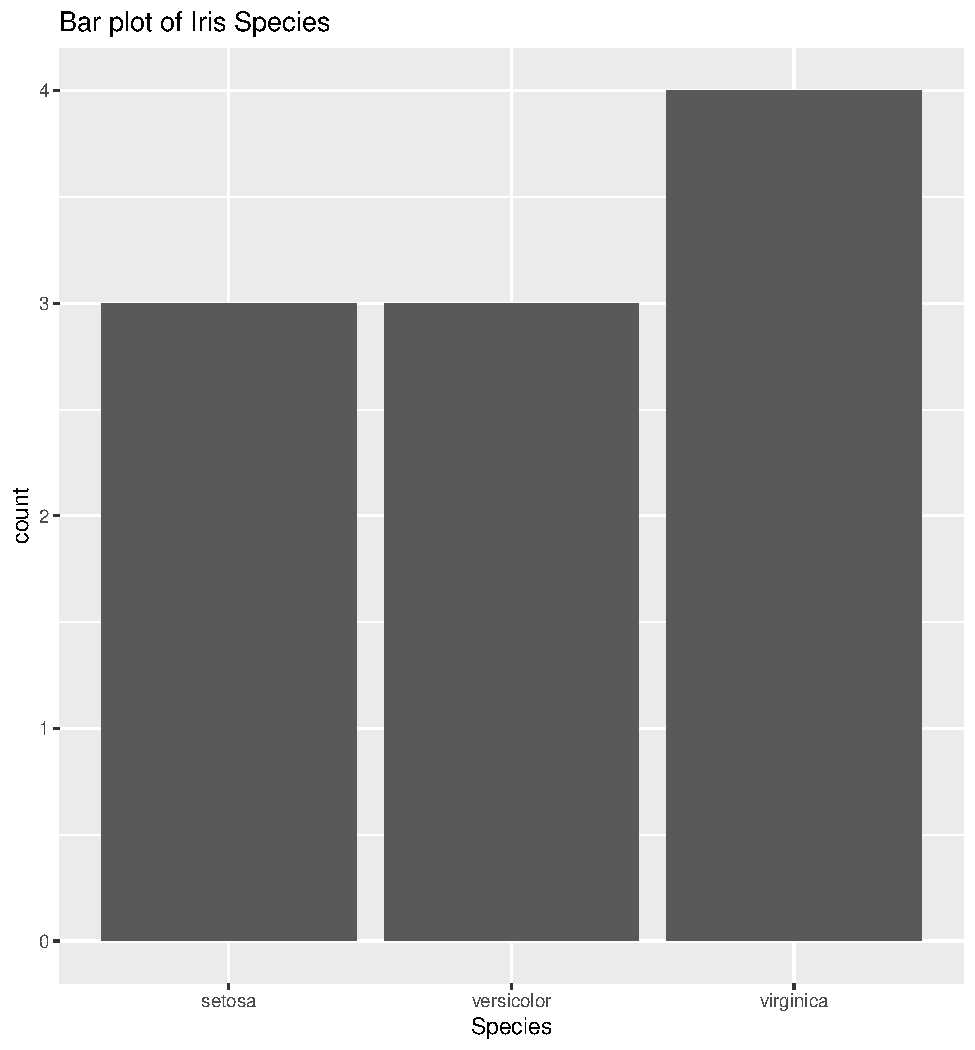
\includegraphics{_main_files/figure-latex/unnamed-chunk-4-1.pdf}

If needed (if you need proportions for the y-axis instead, calculate the
relative frequency table for the frequency table first). Note: again,
this one is missing the total

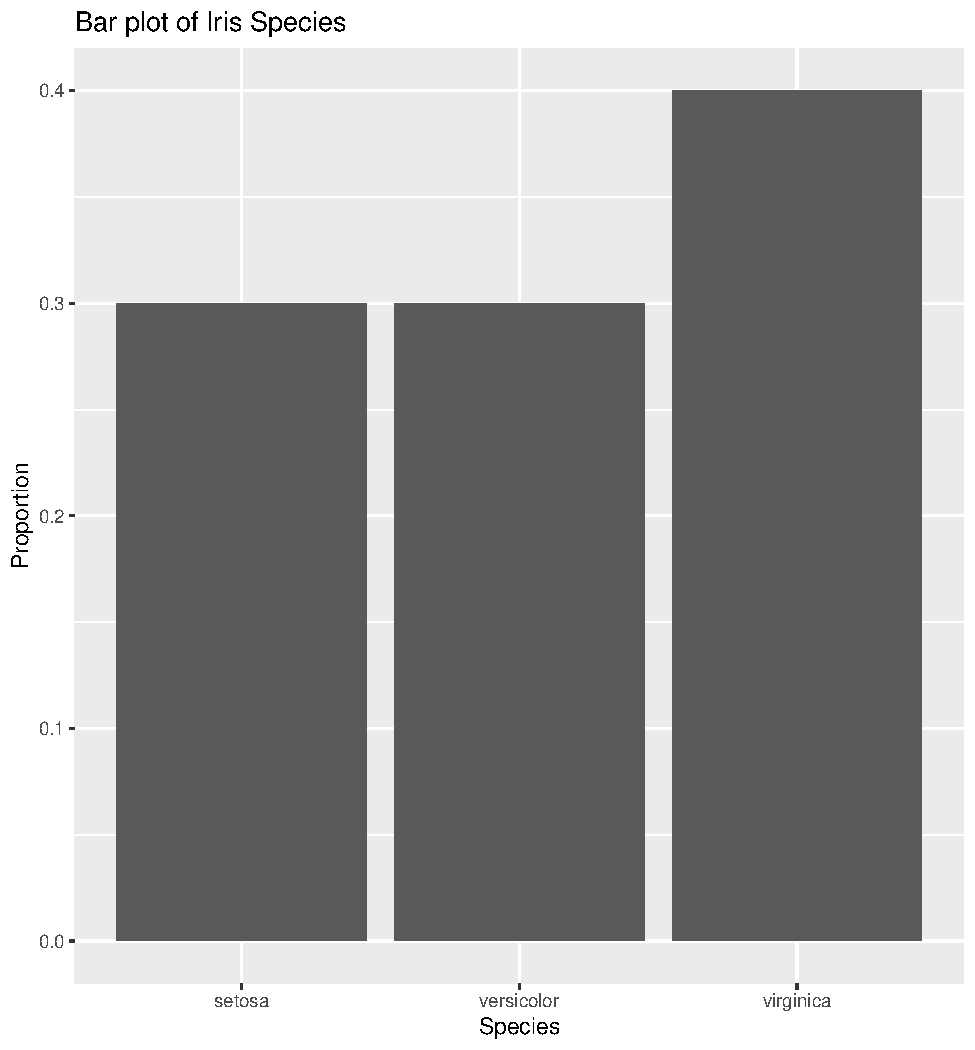
\includegraphics{_main_files/figure-latex/unnamed-chunk-6-1.pdf}

\hypertarget{stacked-bar-plots-and-side-by-side-bar-graphs}{%
\section{Stacked Bar Plots and Side-by-Side Bar Graphs}\label{stacked-bar-plots-and-side-by-side-bar-graphs}}

Stacked bar plots show two categorical variables, one on the
x-axis/y-axis, and the other as the legend (colours). We will call the
variable on the x-axis as the ``groups'' and the variable on the legend as
the ``categories.''

When constructing these bar plots, we first want to determine which
variable goes where (your choice or given choice to you). Then you
calculate relative frequencies \emph{per group}

For example, here I have a two-way table detailing the hair and eye
colour of some statistics students

\begin{verbatim}
## Warning: package 'reshape' was built under R version 4.1.3
\end{verbatim}

\begin{verbatim}
## 
## Attaching package: 'reshape'
\end{verbatim}

\begin{verbatim}
## The following object is masked from 'package:dplyr':
## 
##     rename
\end{verbatim}

\begin{verbatim}
## The following objects are masked from 'package:tidyr':
## 
##     expand, smiths
\end{verbatim}

So if I want eye colour to be my groups, I would calculate the relative
frequencies by column (use the total of the column and divide the whole
column by it), so each group/column will add up to 1.

These numbers will be my bar heights. So for the bar(s) representing
brown eyes:

\begin{itemize}
\item
  black hair will be .3091
\item
  brown hair will be .5409
\item
  red hair will be 0.1182
\item
  blond hair will be 0.0318
\end{itemize}

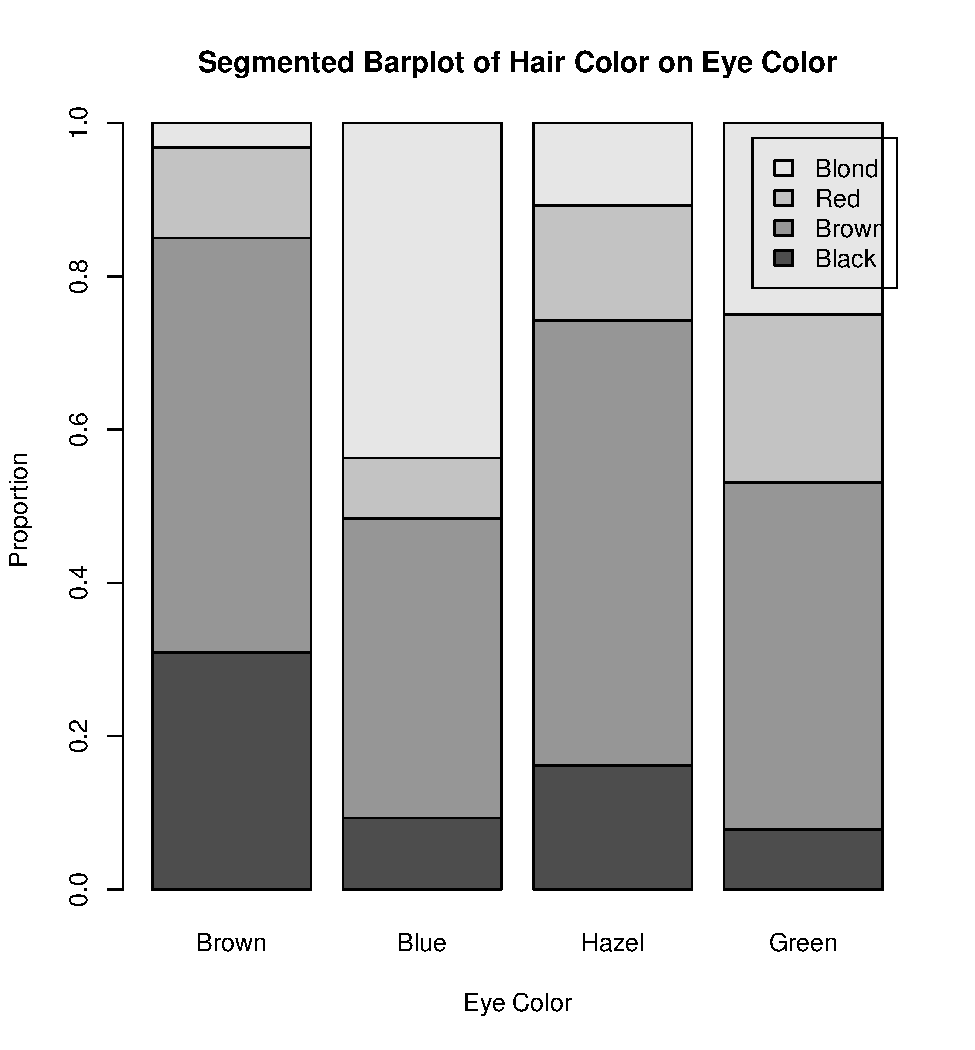
\includegraphics{_main_files/figure-latex/unnamed-chunk-9-1.pdf}

Here's the corresponding side-by-side bar plot. Note that the heights of
the bars are the same as the segmented bar graph.

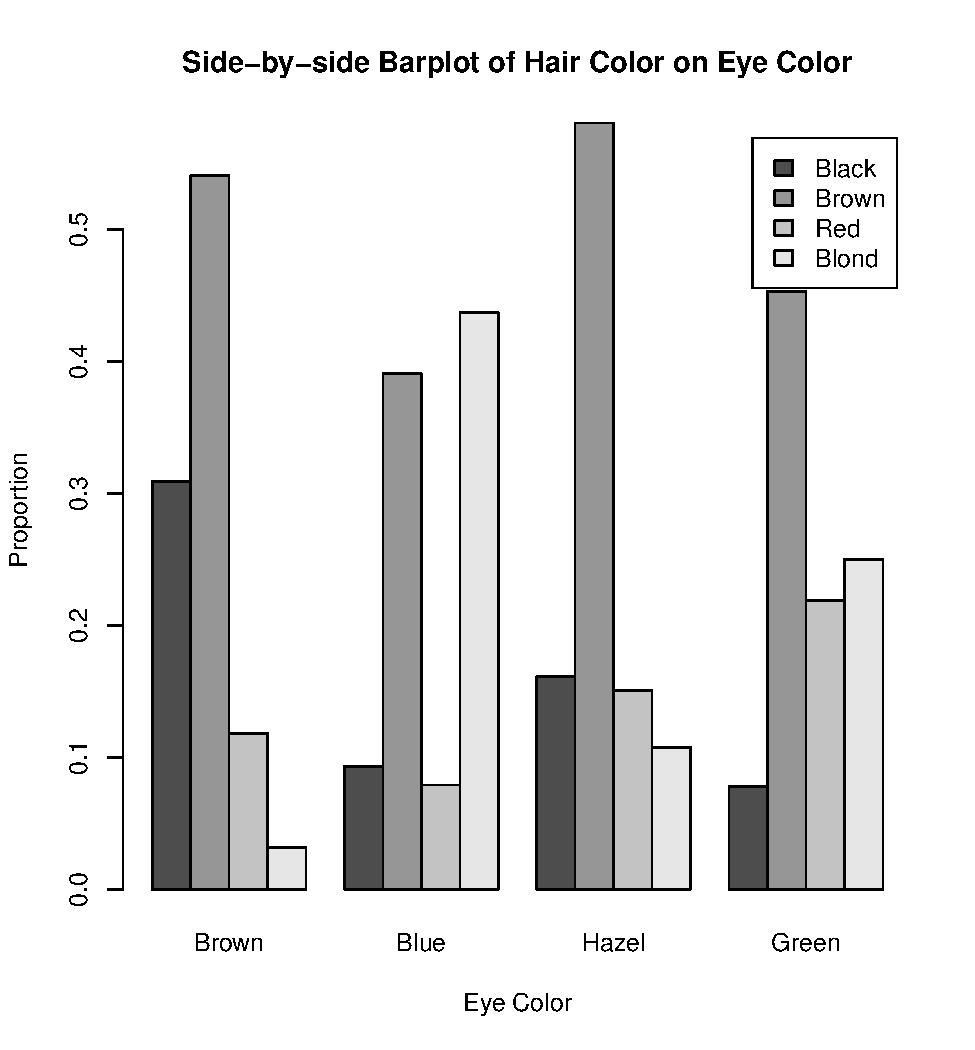
\includegraphics{_main_files/figure-latex/unnamed-chunk-10-1.pdf}

On the other hand, if I want my eye colour to be my groups, I would
calculate the relative frequencies by row (use the total of the row and
divide the whole row by it), so each group/row will add up to 1.

These numbers will be my bar heights. So for the bar(s) representing
black hair:

\begin{itemize}
\item
  brown eyes will be 0.6296296
\item
  blue eyes will be 0.1851852
\item
  hazel eyes will be 0.1388889
\item
  green eyes will be 0.0462963
\end{itemize}

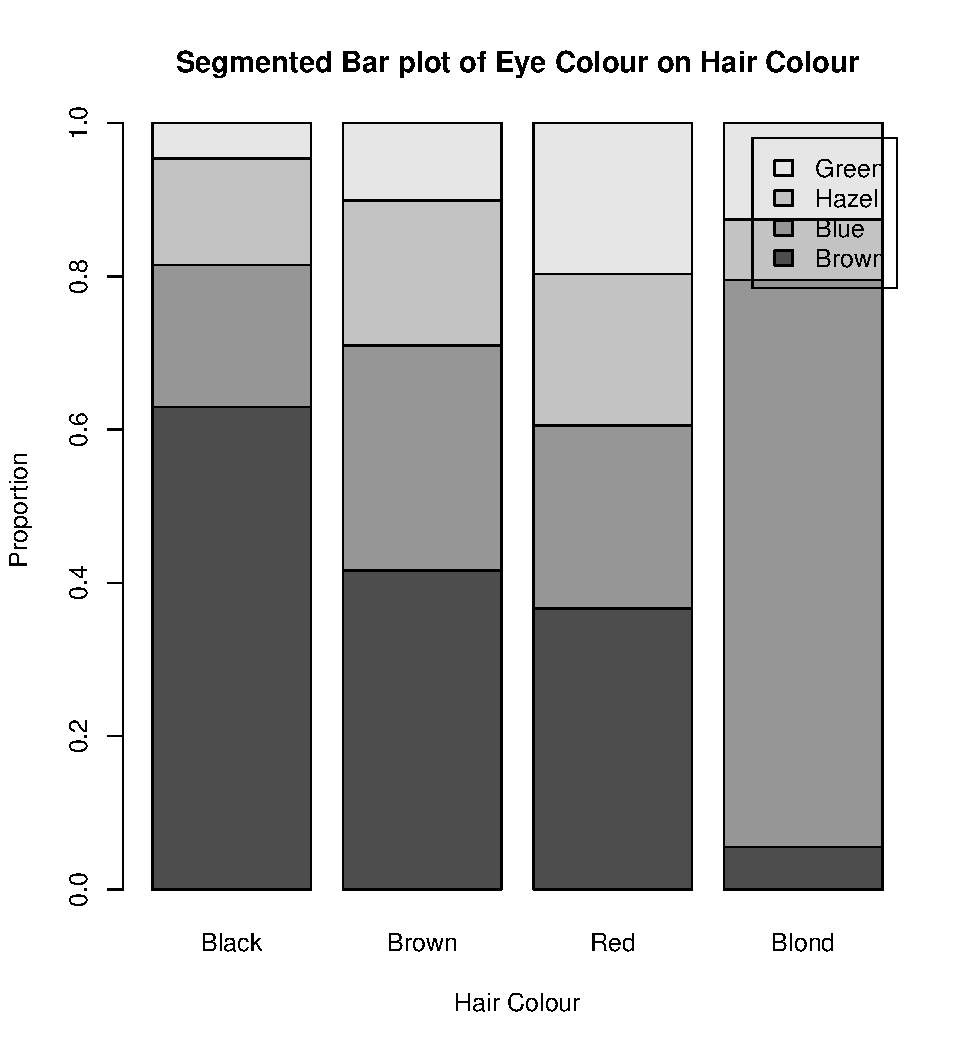
\includegraphics{_main_files/figure-latex/unnamed-chunk-12-1.pdf}

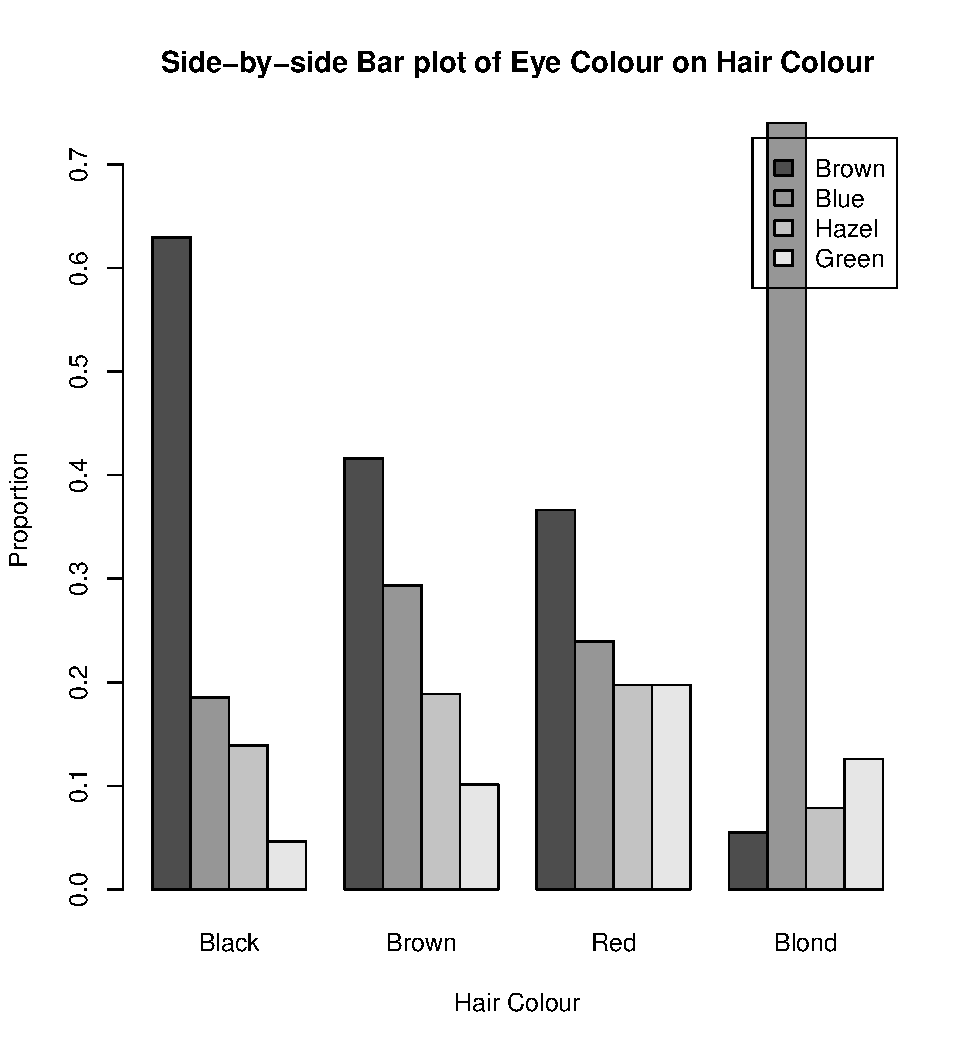
\includegraphics{_main_files/figure-latex/unnamed-chunk-13-1.pdf}

\hypertarget{mosaic-plots}{%
\section{Mosaic Plots}\label{mosaic-plots}}

Mosaic plots are the almost the same as stacked bar plots. The only
difference is that the widths of the bars change according to the
proportion of points in each group. In a mosaic plot, the x-axis will
also measure the proportion of observations/data points within the
groupings (i.e.~the x-axis reflects the marginal distribution of the
variable on the x-axis).

Following the \protect\hyperlink{stacked-bar-plots-and-side-by-side-bar-plots}{same
steps} as the
side-by-side and stacked bar charts to find the heights, we now add an
additional step before plotting.

\emph{Find the widths of the bars by finding the marginal distriubtion of the
variable on the x-axis (the groups)}

\begin{enumerate}
\def\labelenumi{\arabic{enumi}.}
\tightlist
\item
  For each group, find the probability of having that trait. So for
  our previous example, we had this table:
\end{enumerate}

Using our eye colours as the groups (vertical bars), we will find:

\begin{itemize}
\item
  \(P(Brown) \approx .3716\)
\item
  \(P(Blue) \approx .3632\)
\item
  \(P(Hazel) \approx .1571\)
\item
  \(P(Green) \approx .1081\)
\end{itemize}

When we plot our mosaic plot, we do the same thing, except now, we have
our bars differ in widths according to the numbers that we just
calculated.

\hypertarget{quantative-data-visualizations}{%
\chapter{Quantative Data Visualizations}\label{quantative-data-visualizations}}

\hypertarget{dot-plots}{%
\section{Dot Plots}\label{dot-plots}}

Dot plots are for discrete quantitative variables only, and they are
only useful in situations when you have a small range of number so that
you can actually see how the data distribution varies across values.

Dot plots are simple, you draw a number line and then plot points above
the number for each of the number that you see in the data.

Take this data for example:

Now count up each value to figure out how many dots you need at each
value on the number line then plot your graph

\begin{verbatim}
## Bin width defaults to 1/30 of the range of the data. Pick better value with `binwidth`.
\end{verbatim}

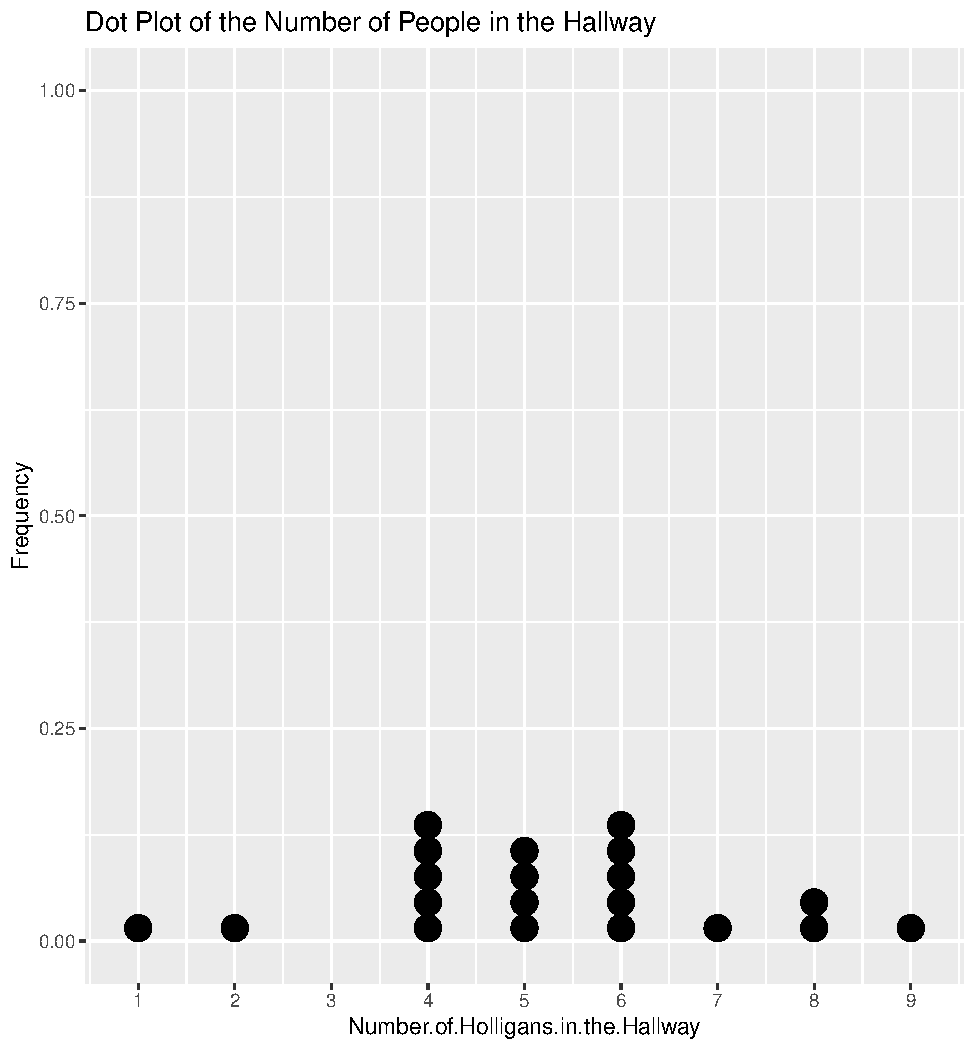
\includegraphics{_main_files/figure-latex/unnamed-chunk-16-1.pdf}

\hypertarget{stemplots}{%
\section{Stemplots}\label{stemplots}}

Using this data as an example, a stem plot looks like this:

A stem plot looks like this:

\begin{verbatim}
## 1 | 2: represents 12
##  leaf unit: 1
##             n: 20
##     0 | 1
##     1 | 8
##     2 | 
##     3 | 36689
##     4 | 4
##     5 | 2339
##     6 | 0228
##     7 | 
##     8 | 19
##     9 | 35
\end{verbatim}

In a stem plot, you need to determine a common ``stem'' of all the numbers
that you're plotting. So if you have integer numbers from 10 to 200,
your stems will be everything from the tens and so on, so you'll have
stems from 1-20. Once you take the stems, you just write the ``leaves''
next to the stem that they belong.

Note that you also have to add a key to show what a stem + leaf means.
The stem and leaves give no information on the decimals in the data, so
as you see above, you need to give an example like (as shown in the
example stemplot):

Key: 1\textbar2 = 12

Here's another example (sorted for convenience)

\begin{verbatim}
## 1 | 2: represents 1.2
##  leaf unit: 0.1
##             n: 50
##    3 | 3
##    3 | 579999
##    4 | 00334
##    4 | 556677788899
##    5 | 00112233444
##    5 | 667888999
##    6 | 234
##    6 | 5
##    7 | 12
\end{verbatim}

\hypertarget{boxplots}{%
\section{Boxplots}\label{boxplots}}

\emph{Also known as a box-and-whisker plot}

Boxplots are primarily made of the \textbf{five number summary} of the data.
The five number summary is made up of the:

\begin{itemize}
\item
  Minimum (min)
\item
  First Quartile (\(Q_1\))
\item
  Median
\item
  Third Quartile (\(Q_3\))
\item
  Maximum (max)
\end{itemize}

To make a simple boxplot, you use the first quartile, median, and third
quartile to make the ``box'' and then use the minimum and maximum to make
the ``whiskers.''

For this simple list of numbers:

Our five number summary is:

\begin{verbatim}
##    Min. 1st Qu.  Median 3rd Qu.    Max. 
##       1       2       4       6       7
\end{verbatim}

As detailed above, our box plot then looks like:

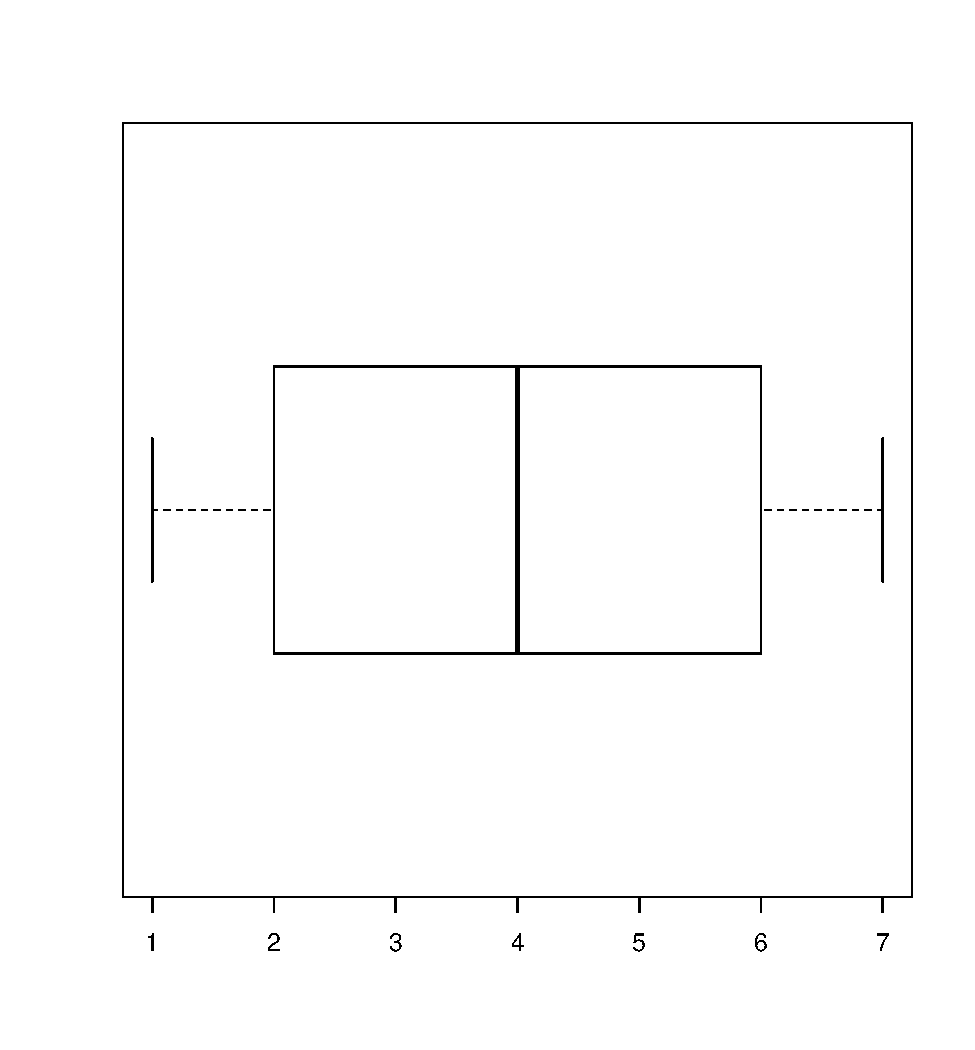
\includegraphics{_main_files/figure-latex/unnamed-chunk-22-1.pdf}

The last detail is that we can calculate outliers using the 1.5 IQR rule
and show them on the boxplot. For either direction (left or right), if
we see outliers in that direction, we only extend the whisker to the
smallest and/or largest point that is not an outlier. Then we plot any
outliers as individual points.

Look at this example data:

Five number summary:

\begin{verbatim}
##    Min. 1st Qu.  Median 3rd Qu.    Max. 
##     -12      -5      -3       0      12
\end{verbatim}

Our numbers calculated by the 1.5 IQR rule are:

\begin{verbatim}
## [1] -12.5   7.5
\end{verbatim}

So our 12 is an outlier. which means we draw our right whisker to 6 and
plot the 12 individually on the number line. Like so:

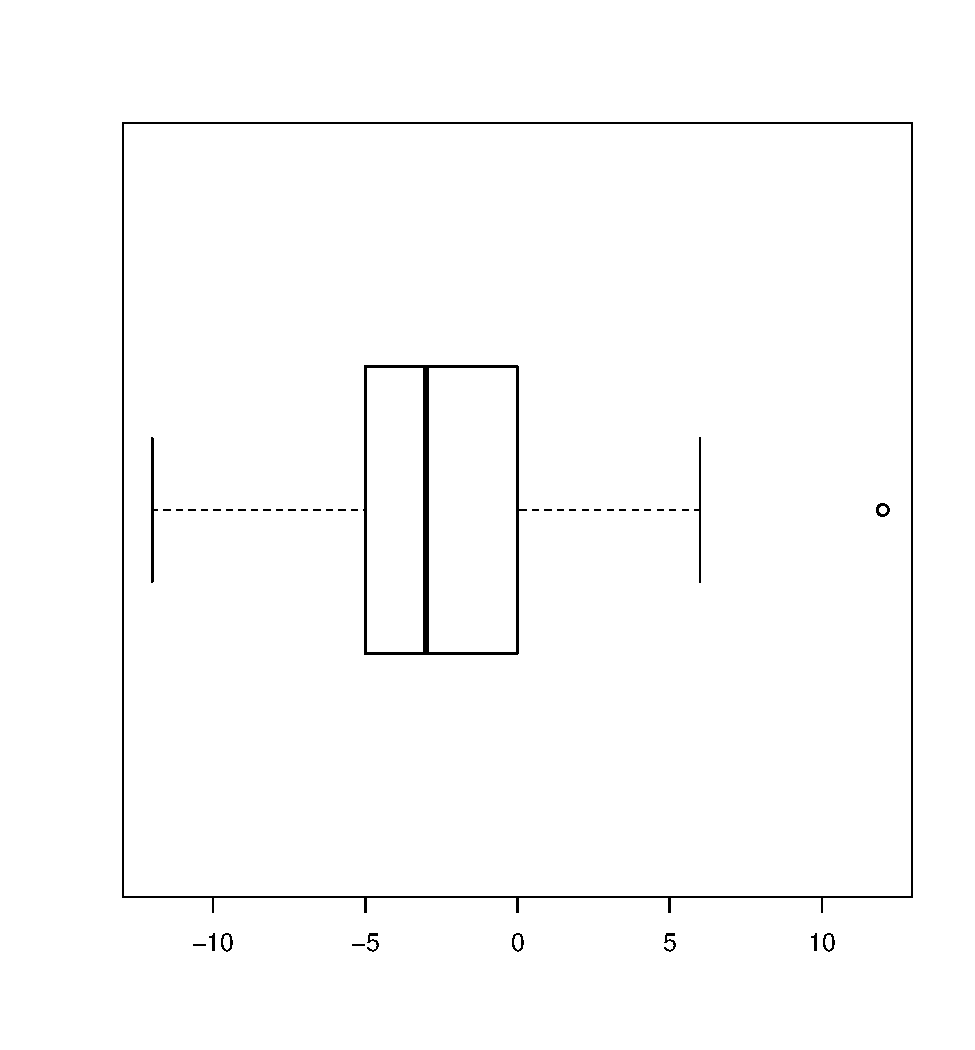
\includegraphics{_main_files/figure-latex/unnamed-chunk-26-1.pdf}

\hypertarget{histograms}{%
\section{Histograms}\label{histograms}}

A histogram is similar to a \protect\hyperlink{bar-plots}{bar plot}, except that
histograms are made for quantitative data and \emph{bars are continuous} in
the sense that there is no gap between bars. To make a histogram, select
an appropriate equal intervals that make it so that you don't have too
many bars and that you don't have too few bars. Your goal with
histograms, as with many other visualizations, is to be able to see the
shape and characteristics of the distribution in question. If you have
too many bars or too few bars, you won't be able to see much important
information (especially think of situations when you have many data
points with very precise decimal measurements).

\begin{enumerate}
\def\labelenumi{\arabic{enumi}.}
\item
  Decide on your intervals (e.g.~by 5's, by 10's, by 100's)
\item
  Within your intervals, count up the number of observations that
  belong in that ``bin''. When you do so, count up observations so that
  you count the left end inclusive and the right end inclusive. So if
  you did intervals of 5, you would do something like counting up
  points \(0 \leq x < 5\), \(5 \leq x < 10\), and so on.
\item
  Plot your bars.
\end{enumerate}

Example:

Consider this example data set:

Our data has this set of summary statistics:

\begin{verbatim}
##        x        
##  Min.   :1.522  
##  1st Qu.:1.912  
##  Median :2.022  
##  Mean   :2.110  
##  3rd Qu.:2.224  
##  Max.   :2.704
\end{verbatim}

With this knowledge, let's make our 7 ``bins'', so let's do these by every
0.2, starting at 1.5 to 2.9. This will be something that you build by
intuition.

Now, count up our values:

\begin{verbatim}
## [1.5,1.7) [1.7,1.9) [1.9,2.1) [2.1,2.3) [2.3,2.5) [2.5,2.7) [2.7,2.9] 
##         1         4         6         5         1         2         1
\end{verbatim}

Now, we just put it together. For each bin, we have a bar and the bars'
heights correspond to the number of individuals in each bin.

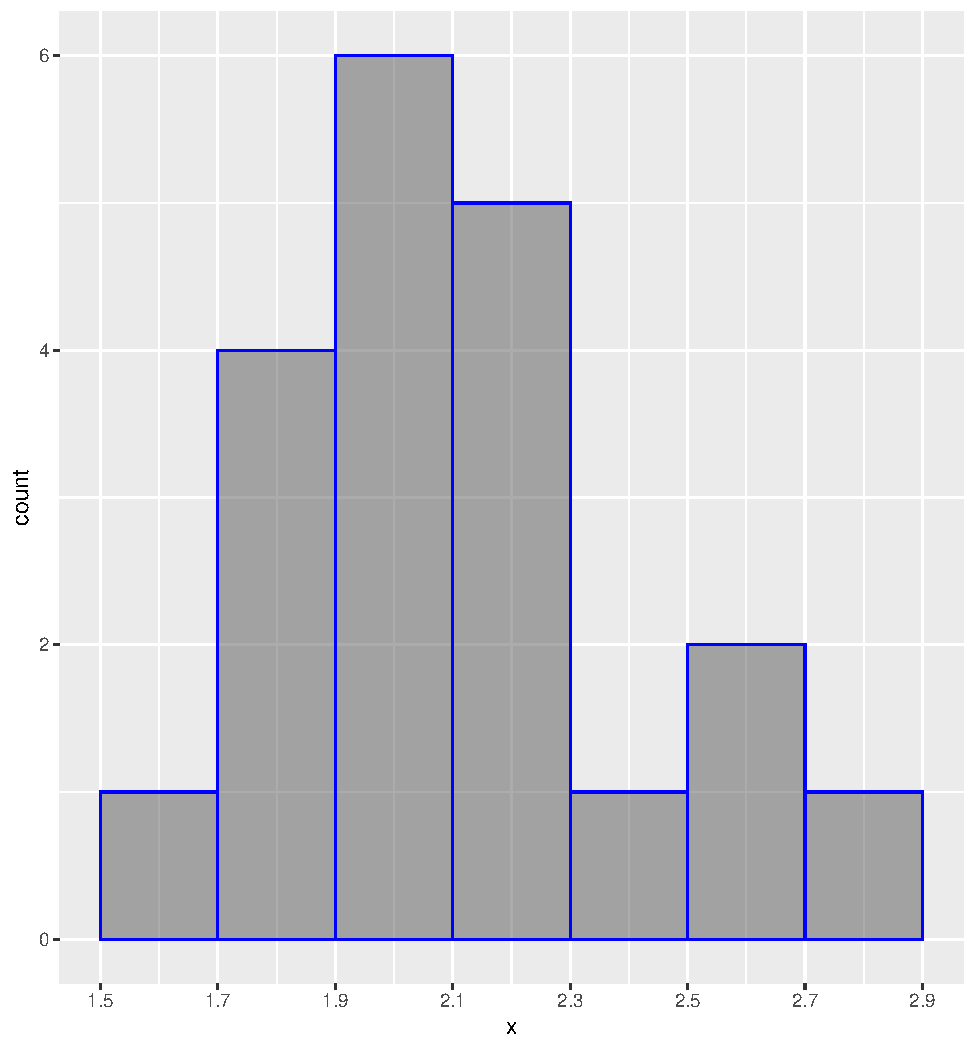
\includegraphics{_main_files/figure-latex/unnamed-chunk-30-1.pdf}

Again, just like bar graphs, we can instead do the relative frequencies
(this is what you'll see most of the time!!!)

\begin{verbatim}
## [1.5,1.7) [1.7,1.9) [1.9,2.1) [2.1,2.3) [2.3,2.5) [2.5,2.7) [2.7,2.9] 
##      0.05      0.20      0.30      0.25      0.05      0.10      0.05
\end{verbatim}

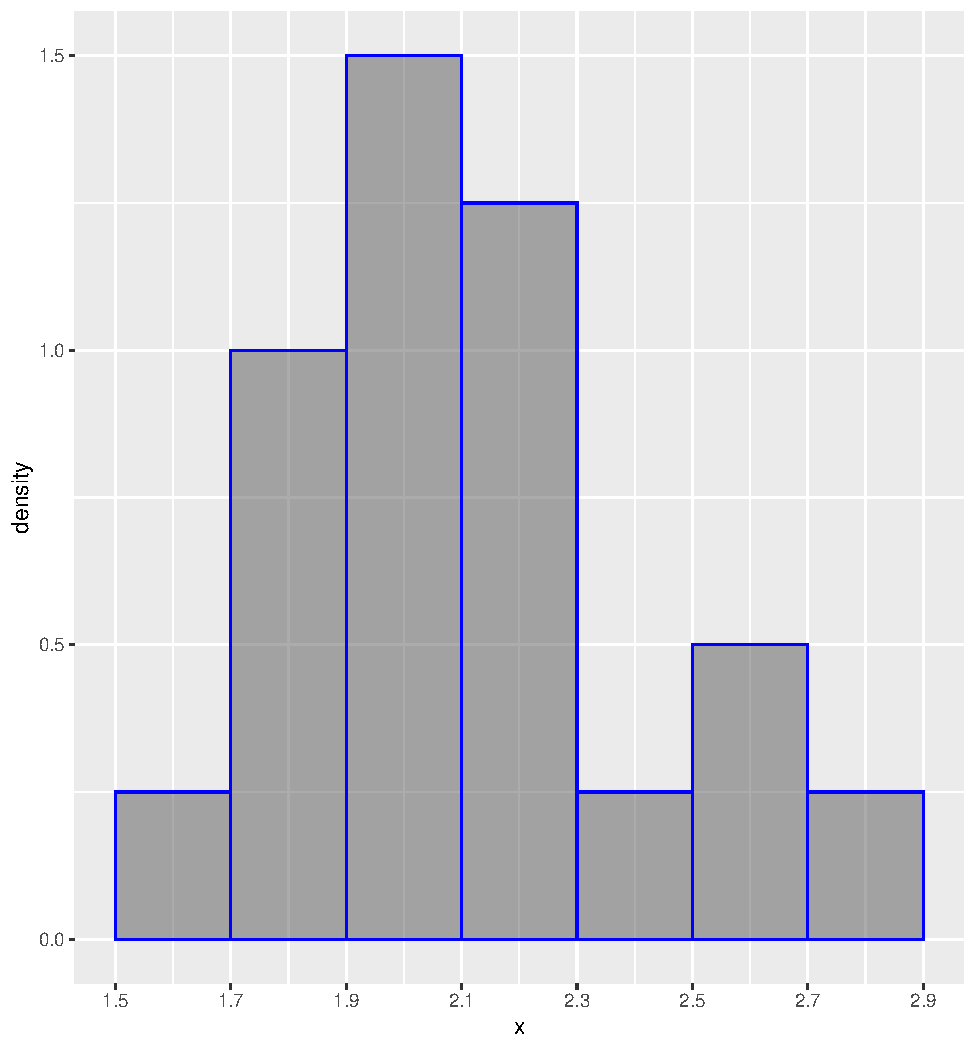
\includegraphics{_main_files/figure-latex/unnamed-chunk-32-1.pdf}

When you have a histogram like this, keep in mind that the bars always
add up to 1 (or 100\%).

\hypertarget{sampling}{%
\chapter{Sampling}\label{sampling}}

When we have a question about a certain population~(an entire group of
individuals). Ideally we would ask them all (take a \textbf{census}). But
contacting every member of a population often isn't very practical: it
would take too much time and cost too much money. Instead, we put the
question to a \textbf{sample}, or subset of individuals of the population
from which we actually collect data, chosen to represent the entire
population.

When you want to identify the population, ask yourself, what does the
question want to know about? What group of people does the
question/problem address?

When identifying the sample, ask yourself, what group does the work done
actually address?

\hypertarget{bias}{%
\section{Bias}\label{bias}}

When we collect data, there is the possibility of the data becoming
systematically pushed towards a specific outcome. For example, if we
want to learn about the GPA average in the school and take a sample of
students only from a class, it's quite possible that the sample is not
representative of the school. We will probably result in a GPA average
that is higher or lower than the actual GPA average in the school. There
are several ways that this can happen. The main way that we learn are:

\hypertarget{response-bias}{%
\subsection{Response Bias}\label{response-bias}}

\hypertarget{non-response-bias}{%
\subsection{Non-response Bias}\label{non-response-bias}}

\hypertarget{voluntary-bias}{%
\subsection{Voluntary Bias}\label{voluntary-bias}}

\hypertarget{experimental-design}{%
\chapter{Experimental Design}\label{experimental-design}}

\hypertarget{probability}{%
\chapter{Probability}\label{probability}}

A process has a valid probability model if and only if:

\begin{itemize}
\tightlist
\item
  Each outcome has a positive probability.
\item
  The sum of all outcomes' probabilities is equal to 1.
\end{itemize}

\hypertarget{density-curves}{%
\chapter{Density Curves}\label{density-curves}}

\hypertarget{random-variables}{%
\chapter{Random Variables}\label{random-variables}}

A \textbf{random variable} is a variable whose value is a numerical outcome
of a random phenomenon.

Random variables can be discrete or continuous. A \textbf{discrete random
variable} \(X\) has a countable, or smaller, number of possible outcomes,
while a \textbf{continuous random variable} \(X\) can take on an infinite
number (theoretically) of different values.

The \textbf{probability distribution} of a random variable \(X\) gives us all
possible values of \(X\), and their corresponding probabilities.
Probability distributions are typically given as tables, histograms
(with probability on the y-axis, instead of frequency), or density
curves (like the Normal curve).

\hypertarget{discrete-random-variables}{%
\section{Discrete Random Variables}\label{discrete-random-variables}}

A discrete random variable describes a process that only has specific,
predefined outcomes. For example, you can be finding the probability of
people having blue, brown, and black eyes. Or you can be finding the
probability of people earning salaries in the ranges of \textless\$30,000,
\$30,000 - \$50,000, \$50,000 - \$ 70,000, \$70,000 - \$ 100,000,
\textgreater\$100,000.

When we have a discrete random variable \(X\) whose probability
distribution is

\[
\begin{aligned}
    \textbf{Value:}& ~~~~ x_1 ~~~~ x_2 ~~~~ x_3 ~~~~ \cdots \\
    \textbf{Probability:}& ~~~~ p_1 ~~~~ p_2 ~~~~ p_3 ~~~~\cdots
\end{aligned}
\]

we know the following about the mean and standard deviation of \(X\):

\[\mu_X = E(X) = \sum x_i P(x_i)\]

\[\sigma_X = \sqrt{\sum \left( x_i - \mu_X \right) ^2 P \left( x_i \right)}\]

Keep in mind that the standard deviation formula here (and else
where) is equivalent to the formula of population standard deviation
when we divide by \(n\) instead of multiplying by \(P(x_i)\).

\[
\begin{aligned}
\sigma_X &= \sqrt{\frac{\sum(x_i - \mu_X)^2}{n}} \\
&=\sqrt{E((X - \bar x)^2)} \\
&=\sqrt{\sum \left( x_i - \mu_X \right) ^2 P \left( x_i \right)}\\
\end{aligned}
\]

In other words, remember that we define standard deviation as the root
mean square of the squared differences from the mean. Since we are
taking the mean of the squared differences from the mean in both
formulas (I use the definition for mean from step 1 to 2 and the
definition of mean for discrete variables from step 2 to 3), the two
formulas are equivalent.

The variance of a random variable \(X\) is:

\[
Var(X) = \sigma_X^2
\]

\hypertarget{binomial-random-variables}{%
\subsection{Binomial Random Variables}\label{binomial-random-variables}}

Binomial random variables have parameters \(n\) and \(p\), and can be
written \(B(n, p)\). Remember, Normal random variables have parameters and
and can be written \(N(\mu,\sigma)\).

The pdf of a Binomial Random Variable (i.e.~the binomial formula) is:

\[
\begin{aligned}
    P(X=k) &= {n \choose k} p^k (1-p)^{n-k}\\
    \text{where } k &= 0, 1, 2, 3, \cdots, n
\end{aligned}
\]

To apply this formula in a graphing calculator:
\(\texttt{2nd -> vars (distr) -> binompdf}\)

Usage: \(\texttt{binompdf(n, p[,x])}\)

The cdf of a Binomial Random Variable is: \[
\begin{aligned}
    P(X\leq k) &= \sum_{i = 0}^n {n \choose i} p^i (1-p)^{n-i}
\end{aligned}
\]

In graphing calculator: \(\texttt{2nd -> vars (distr) -> binomcdf}\)

Usage: \(\texttt{binomcdf(n, p[,x])}\)

The mean and standard deviation of a binomial random variable is given
by:

\[
\begin{aligned}
    \mu_X &= n p \\
    \sigma_X &= \sqrt{n p q} \\
    &\text{, where } q = 1-p.
\end{aligned}
\]

\hypertarget{binomial-setting}{%
\subsubsection{Binomial setting}\label{binomial-setting}}

We can identify a binomial setting when we know:

\begin{enumerate}
\def\labelenumi{\arabic{enumi}.}
\item
  \textbf{B}inary? The possible outcomes of each trial can be classified as
  ``success'' or ``failure'' (in our case rolling a 7 or not).
\item
  \textbf{I}ndependent? Trials must be independent; that is, knowing the
  result of one trial must not tells us anything about the result of
  another trial.
\item
  \textbf{N}umber? The number of trials n of the chance process must be
  fixed in advance. (this was 5, then 100).
\item
  \textbf{S}ame? There is the same probability p of success on each trial
  (1/6).
\end{enumerate}

\hypertarget{condition}{%
\subsubsection{10\% Condition}\label{condition}}

The second condition is often not perfectly met, as in the case of an
SRS from some population. Imagine choosing 10 students from a class of
15 females and 15 males---as we choose people, the remaining population
changes, which changes the probability that the next person chosen will
be male or female.

When we lack complete independence, we can see the consequence of this
is negligible as long as our sample is small relative to the population
from which we are sampling. If we were choosing our 10 people from a
school of 3,300 students, the change in probability from person to
person would be small enough to ignore.

The general rule is that the sample needs to be less than
\(\frac{1}{10}\), or 10\%, of the population. We refer to this as the 10\%
condition.

\[n \leq (.10) N\]

\hypertarget{normal-approximation-to-the-binomial-distribution}{%
\subsubsection{Normal Approximation to the Binomial Distribution}\label{normal-approximation-to-the-binomial-distribution}}

Remember that as \(n\) gets large, a binomial random variable \(X\) can take
on more and more different values, and it can become tedious to continue
to treat X as a discrete random variable. As \(n\) get larger, we can
treat \(X\) as a continuous random variable, more specifically:

As \(n\) gets larger, the binomial distribution gets closer to a normal
distribution. However, before we use a normal distribution to
approximate a binomial distribution, we have to check the following
condition:

\hypertarget{large-counts-condition}{%
\paragraph{Large Counts condition}\label{large-counts-condition}}

If \(np \geq 10\) and \(n(1-p) \geq 10\), then we can use a Normal
distribution to model a binomial distribution. In other words, if the
expected number of successes and failures (respectively) is greater than
or equal to 10.

\hypertarget{doing-a-normal-approximation}{%
\paragraph{Doing a normal approximation}\label{doing-a-normal-approximation}}

First verify all the conditions for a Binomial setting and the Large
Counts Condition. Since we know that we have a binomial setting, we then
know the distribution that we want to use is \(Normal(np, \sqrt{npq})\) proceed with the calculations according to this distribution.

\hypertarget{geometric-random-variables}{%
\subsection{Geometric Random Variables}\label{geometric-random-variables}}

If \(X \sim G(p)\), in other words, if \(X\) has a geometric distribution
with parameter \(p\), the pdf of a geometric random variable is:

\[
\begin{aligned}
    P(X=x) &= (1-p)^{x-1}p\\
    \text{where } x &= 1, 2, 3, \cdots
\end{aligned}
\]

In graphing calculator: \(\texttt{2nd -> vars (distr) -> geometpdf}\)

Usage: \(\texttt{geometpdf(p, x)}\)

The cdf of a Geometric Variable is:

\[
\begin{aligned}
    P(X\leq x) &= \sum_{i=1}^x(1-p)^{i-1}p
\end{aligned}
\]

In graphing calculator: \(\texttt{2nd -> vars (distr) -> geometcdf}\)

Usage: \(\texttt{geometcdf(p, x)}\)

The mean and standard deviation of a geometric random variable is given
by:

\[
\begin{aligned}
    \mu_X &= \frac{1}{p} \\
    \sigma_X &= \frac{\sqrt{q}}{p} \\
    &\text{, where } q = 1-p.
\end{aligned}
\]

\hypertarget{the-geometric-setting}{%
\subsubsection{The Geometric Setting}\label{the-geometric-setting}}

A geometric setting is very similar to a binomial setting, except that
\textbf{n, the number of trials is not fixed}.

A geometric setting is defined as a series of observations where these 4
conditions are met:

\begin{enumerate}
\def\labelenumi{\arabic{enumi}.}
\item
  \textbf{B}inary? The Possible outcomes of each trial can be classified as
  ``success'' or ``failure''
\item
  \textbf{I}ndependent? Trials must be independent, that is, knowing the
  result of one trial must not have any effect on the result of any
  other trial.
\item
  \textbf{T}rials? The goal is to count the number of trials until the
  first success occurs.
\item
  \textbf{S}uccess? On each trial, the probability p of success must be the
  same.
\end{enumerate}

\hypertarget{operations-with-random-variables}{%
\section{Operations with Random Variables}\label{operations-with-random-variables}}

\hypertarget{constants}{%
\subsection{Constants}\label{constants}}

When we add a constant \(a\) and/or multiply by a constant \(b\) to a random
variable \(X\), we perform a linear transformation of the form

\[
a + bX
\]

The mean of the transformed variable is:

\[
\mu_{a+bX}=a+\mu_{bX}=a+b\mu_X
\]

The standard deviation of the transformed variable is:

\[
\sigma_{a+bX}=\sigma_{bX}=b\sigma_X
\]

\hypertarget{random-variables-1}{%
\subsection{Random Variables}\label{random-variables-1}}

In general, we can describe the mean and standard deviation of the sum
or difference of independent random variables with these formulas:

\[\mu_{X \pm Y} = \mu_X \pm \mu_Y\]

\textbf{If the random variables \(X\) and \(Y\) are independent}, then

\[ \sigma_{X \pm Y}^2 = \sigma_X^2 + \sigma_Y^2 \]

\hypertarget{sampling-distributions}{%
\chapter{Sampling distributions}\label{sampling-distributions}}

\hypertarget{confidence-intervals}{%
\chapter{Confidence Intervals}\label{confidence-intervals}}

A \textbf{Confidence Interval} is an interval of plausible values for the population parameter and is used to estimate the parameter. The interval is calculated from the data and has the form

\[\text{point estimate} ± \text{margin of error}\]

Margin of errors are calculated from the confidence level and the data and has the form

\[ME = m = \text{critical value} \cdot \text{standard error of the statistic}\]

The difference between the point estimate, the value of the statistics from a sample that provides an estimate of the population parameter, and the true parameter value will be less than the margin of error in C\% of samples.

\hypertarget{interpreting-confidence-intervals}{%
\section{Interpreting Confidence Intervals}\label{interpreting-confidence-intervals}}

You can say something of the form:

I am {[}confidence level{]}\% confident the interval from {[}lower bound{]} to {[}upper bound{]} captures the {[}true parameter in the context of the problem{]}.

You CANNOT say that ``There is a 95\% chance that this interval contains the population (proportion or mean)'' because your single interval either did or did not capture the real value, and either has a probability of 0 or 1

\hypertarget{interpreting-confidence-level}{%
\section{Interpreting Confidence Level}\label{interpreting-confidence-level}}

If we take many, many samples and create many, many intervals using the same method, about {[}confidence level{]}\% of them will capture the {[}true parameter in the context of the problem{]}.

In other words, you can say that: ``95\% of intervals created in this manner will capture the true population (proportion or mean)''

\hypertarget{changing-confidence-levels}{%
\section{Changing Confidence Levels}\label{changing-confidence-levels}}

When we increase confidence level, we are saying that more intervals in this manner should capture the true parameter. This means that to increase confidence level means that the confidence intervals need to increase in width.

When we increase the size of a sample, the precision of our statistic increases because of the reduction in sampling variability (standard deviation of the statistic decreases as n increases). This means that we can now guess/estimate a smaller range compared to if we had a smaller sample size. So, when we increase the size of our samples, our confidence intervals will have smaller widths compared to those with a smaller sample size.

\hypertarget{conditions-for-confidence-intervals}{%
\section{Conditions for Confidence Intervals}\label{conditions-for-confidence-intervals}}

\hypertarget{the-data-must-come-from-a-random-sample-or-random-assignment-in-an-experiment.}{%
\subsection*{1. The data must come from a random sample, or random assignment in an experiment.}\label{the-data-must-come-from-a-random-sample-or-random-assignment-in-an-experiment.}}

In order to infer about a larger population, we must have a random, unbiased sample from that population. If the sample is not random, we need to think about whether it's at least unbiased and/or representative. If so, we may be able to treat it as a random sample, but we must state that we're doing this. If you're not told that a sample is random, you can write something like ``I'm going to have to assume I can treat this as a random sample''.

In the case of experiments, we can perform statistical tests on the data from our experimental groups, even if we don't have a random sample from a larger population. In this case, we must make sure we have internal validity in our experiment (a well-conducted experiment with control, replication, and random assignment of treatments). If we do, our results are valid for our subjects, but we may or may not be able to generalize to a larger population. This depends on whether our subjects are a random sample from, or at least representative of, some larger population.

\hypertarget{the-sample-must-be-large-enough}{%
\subsection*{2. The sample must be large enough}\label{the-sample-must-be-large-enough}}

\hypertarget{proportions}{%
\subsubsection*{Proportions}\label{proportions}}

For proportions, remember, the population is never anywhere near normal (it's always two bars, yes and no). In this case we check the \emph{Large Counts Condition}; that both of the following are true:

\(np ≥ 10\) (expected \# of successes is at least 10)

\(n(1-p) ≥ 10\) (expected \# of failures is at least 10)

This ensures that our sample proportion can take on enough different values (and make enough bars in a histogram) to create an approximately normal sampling distribution.

\hypertarget{sample-means}{%
\subsubsection*{Sample means}\label{sample-means}}

In the case of sample means, the sampling distribution is approximately normal if at least one of the following conditions are met.

\emph{Normal/Large Condition}

-The population from which we are sampling is approximately Normal.

-Our sample size is sufficiently large (\(n > 30\))

When \(n<30\)

-Graph of the sample data does not show any strong skew or outliers.

\hypertarget{observations-in-our-sample-must-be-independent}{%
\subsection*{3. Observations in our sample must be independent}\label{observations-in-our-sample-must-be-independent}}

In random samples from a population, observations are never independent because the population changes with every person we sample and remove from it. However, this effect is small enough to ignore as long as the population from which we're sampling is at least 10 times as large as our sample (\emph{i.e.~the 10\% Condition}) . This needs to be stated!

In experiments, or other situations where we're not sampling from a population (rolls of dice for example), we just need to think about whether the outcome of one observation could be having any effect on the outcome of another observation. Often we don't know this, so we need to state that we're assuming it; ''I'm going to have to assume I can treat these observations as independent''.

\hypertarget{one-sample-z-intervals}{%
\section{One-Sample z-Intervals}\label{one-sample-z-intervals}}

A \(C\)\% confidence interval for the unknown population proportion \(p\) when all conditions are met is calculated with the following:

\[\hat p \pm z^* \sqrt{\frac{\hat p (1 - \hat p)}{n}}\]

where \(z^*\) is the critical value for the standard Normal curve with \(C\)\% of its area between \(-z^*\) and \(z^*\) and the standard error of the sample proportion is \(SE_{\hat p}=\sqrt{\frac{\hat p (1 - \hat p)}{n}}\)

\hypertarget{one-sample-t-intervals}{%
\section{One-Sample t-Intervals}\label{one-sample-t-intervals}}

A \(C\)\% confidence interval for the unknown population mean \(\mu\) when all conditions are met is calculated with the following:

\[\bar x \pm t^* \frac{s_x}{\sqrt{n}}\]

where \(t^*\) is the critical value for the Student's \(t\) distribution corresponding with degrees of freedom \(df = n - 1\) with \(C\)\% of its area between \(-t^*\) and \(t^*\) and the standard error of the sample mean is \(SE_{\bar x}=\frac{s_x}{\sqrt{n}}\).

\hypertarget{the-four-step-process}{%
\section{The Four-Step Process}\label{the-four-step-process}}

\begin{enumerate}
\def\labelenumi{\arabic{enumi}.}
\tightlist
\item
  \textbf{STATE} exactly what you're doing
\end{enumerate}

Be sure to be specific here, especially with regard to defining the actual numbers you will be analyzing. You need to demonstrate your understanding of the population about which you're inferring, the procedure you're using, and the parameter of interest. If you're conducting a statistical test (which we'll cover next), you also need to write hypotheses here. For example: ``I want to estimate the true proportion of all CA voters that support a repeal of Prop 8 with 95\% confidence''

\begin{enumerate}
\def\labelenumi{\arabic{enumi}.}
\setcounter{enumi}{1}
\tightlist
\item
  \textbf{PLAN} which method you will use and that the necessary conditions are met.
\end{enumerate}

If the conditions are not met, or if you can't be sure they're met, you need to explain what needs to be true in order for the conditions to be met.

\begin{enumerate}
\def\labelenumi{\arabic{enumi}.}
\setcounter{enumi}{2}
\tightlist
\item
  \textbf{DO} the calculations
\end{enumerate}

Perform the calculations necessary for the method you chose to use. Show all work!

\begin{enumerate}
\def\labelenumi{\arabic{enumi}.}
\setcounter{enumi}{3}
\tightlist
\item
  \textbf{CONCLUDE} in the context of the situation by giving a complete explanation of the value(s) you calculated in (c).
\end{enumerate}

``I am 95\% confident that the true proportion of all CA voters that support a repeal of Prop 8 is between 42\% and 51\%. 95\% of intervals created like this one will capture the true population proportion of CA voters that support a repeal of Prop 8.''

\hypertarget{hypothesis-testing}{%
\chapter{Hypothesis Testing}\label{hypothesis-testing}}

\hypertarget{linear-regression}{%
\chapter{Linear Regression}\label{linear-regression}}

\hypertarget{appendix-appendix}{%
\appendix}


\hypertarget{ap-exam-formula-sheet}{%
\chapter{AP Exam Formula Sheet}\label{ap-exam-formula-sheet}}

\hypertarget{i.-descriptive-statistics}{%
\section{I. Descriptive Statistics}\label{i.-descriptive-statistics}}

\[
\begin{aligned}
\bar x &= \frac{1}{n}\sum x_i = \frac{\sum x_i}{n} \\\\
s_x &= \sqrt{\frac{1}{n-1}\sum (x_i - \bar x)^2} = \sqrt{\frac{\sum(x_i -\bar x)^2}{n - 1}}\\\\
\hat y &= a + bx \\\\
\bar y &= a + b \bar x\\\\
r &= \frac{1}{n-1}\sum \left( \frac{x_i - \bar x}{s_x}\right) \left( \frac{y_i -\bar y}{s_y}\right)\\\\
b &= r \frac{s_y}{s_x}
\end{aligned}
\]

\hypertarget{ii.-probability-and-distributions}{%
\section{II. Probability and Distributions}\label{ii.-probability-and-distributions}}

\[
\begin{aligned}
P(A \cup B) &= P(A) + P(B) - P(A \cap B) \\\\
P(A | B) &= \frac{P(A \cap B)}{P(B)}
\end{aligned}
\]

\begin{longtable}[]{@{}
  >{\raggedright\arraybackslash}p{(\columnwidth - 4\tabcolsep) * \real{0.5464}}
  >{\raggedright\arraybackslash}p{(\columnwidth - 4\tabcolsep) * \real{0.1821}}
  >{\raggedright\arraybackslash}p{(\columnwidth - 4\tabcolsep) * \real{0.2714}}@{}}
\toprule()
\begin{minipage}[b]{\linewidth}\raggedright
Probability Distribution
\end{minipage} & \begin{minipage}[b]{\linewidth}\raggedright
Mean
\end{minipage} & \begin{minipage}[b]{\linewidth}\raggedright
Standard Deviation
\end{minipage} \\
\midrule()
\endhead
Discrete random variable, \(X\) & \(\mu_X = E(X) = \sum x_i P(x_i)\) & \(\sigma_X = \sqrt{\sum \left( x_i - \mu_X \right) ^2 P \left( x_i \right)}\) \\
If \(X\) has a \textbf{binomial distribution} with parameters \(n\) and \(p\), then: \(P(X = x) = {n \choose x} p^x (1 - p)^{n - x}\) where \(x = 0, 1, 2, 3, ..., n\) & \(\mu_X = np\) & \(\sigma_X = \sqrt{np(1-p)}\) \\
If \(X\) has a \textbf{geometric distribution} with parameter \(p\), then: \(P(X = x) = (1 - p)^{x - 1} p\) where \(x = 1, 2, 3, ...\) & \(\mu_X = \frac{1}{p}\) & \(\sigma_X = \frac{\sqrt{1-p}}{p}\) \\
\bottomrule()
\end{longtable}

\hypertarget{iii.-sampling-distributions-and-inferential-statistics}{%
\section{III. Sampling Distributions and Inferential Statistics}\label{iii.-sampling-distributions-and-inferential-statistics}}

\[\text{Standardized test statistic:}~~~~ \frac{\text{statistic} - \text{parameter}} {\text{standard error of the statistic}}\]\\

\[\text{Confidence interval:}~~~~ \text{statistic} \pm (\text{critical value}) (\text{standard error of statistic})\]\\

\[\text{Chi-square statistic:}~~~~ \chi^2 = \sum \frac{(\text{observed} - \text{expected})^2}{\text{expected}}\]

\hypertarget{sampling-distributions-for-proportions}{%
\subsection{Sampling distributions for proportions:}\label{sampling-distributions-for-proportions}}

\begin{longtable}[]{@{}
  >{\raggedright\arraybackslash}p{(\columnwidth - 6\tabcolsep) * \real{0.0996}}
  >{\raggedright\arraybackslash}p{(\columnwidth - 6\tabcolsep) * \real{0.0932}}
  >{\raggedright\arraybackslash}p{(\columnwidth - 6\tabcolsep) * \real{0.1864}}
  >{\raggedright\arraybackslash}p{(\columnwidth - 6\tabcolsep) * \real{0.6208}}@{}}
\toprule()
\begin{minipage}[b]{\linewidth}\raggedright
Random Variable
\end{minipage} & \begin{minipage}[b]{\linewidth}\raggedright
Parameters of Sampling Distribution (mean)
\end{minipage} & \begin{minipage}[b]{\linewidth}\raggedright
Parameters of Sampling Distribution (standard deviation)
\end{minipage} & \begin{minipage}[b]{\linewidth}\raggedright
Standard Error* of Sample Statistic
\end{minipage} \\
\midrule()
\endhead
For one population: \(\hat p\) & \(\mu_{\hat p} = p\) & \(\sigma_{\hat p} = \sqrt{\frac{p(1-p)}{n}}\) & \(s_{\hat p} = \sqrt{\frac{\hat p (1 - \hat p)}{n}}\) \\
For two populations:\(\hat p_1 - \hat p_2\) & \(\mu_{\hat p_1 - \hat p_2} = p_1 - p_2\) & \(\sigma_{\hat p_1 - \hat p_2}= \sqrt{\frac{p_1(1-p_1)}{n_1} + \frac{p_2(1-p_2)}{n_2}}\) & \(s_{\hat p_1 - \hat p_2}= \sqrt{\frac{\hat p_1(1- \hat p_1)}{n_1} + \frac{\hat p_2(1- \hat p_2)}{n_2}}\)When \(p_1 = p_2\) is assumed:\(s_{\hat p_1 -\hat p_2} = \sqrt{\hat p_c (1 - \hat p_c) \left( \frac{1}{n_1} + \frac{1}{n_2} \right)}\)where \(\hat p_c = \frac{X_1 + X_2}{n_1 + n_2}\) \\
\bottomrule()
\end{longtable}

\hypertarget{sampling-distributions-for-means}{%
\subsection{Sampling distributions for means:}\label{sampling-distributions-for-means}}

\begin{longtable}[]{@{}
  >{\raggedright\arraybackslash}p{(\columnwidth - 6\tabcolsep) * \real{0.1843}}
  >{\raggedright\arraybackslash}p{(\columnwidth - 6\tabcolsep) * \real{0.1765}}
  >{\raggedright\arraybackslash}p{(\columnwidth - 6\tabcolsep) * \real{0.3490}}
  >{\raggedright\arraybackslash}p{(\columnwidth - 6\tabcolsep) * \real{0.2902}}@{}}
\toprule()
\begin{minipage}[b]{\linewidth}\raggedright
Random Variable
\end{minipage} & \begin{minipage}[b]{\linewidth}\raggedright
Parameters of Sampling Distribution (mean)
\end{minipage} & \begin{minipage}[b]{\linewidth}\raggedright
Parameters of Sampling Distribution (standard deviation)
\end{minipage} & \begin{minipage}[b]{\linewidth}\raggedright
Standard Error* of Sample Statistic
\end{minipage} \\
\midrule()
\endhead
For one population: \(\overline{X}\) & \(\mu_{\overline X} = \mu\) & \(\sigma_{\overline X} = \frac{\sigma}{\sqrt n}\) & \(s_{\overline X} = \frac{s}{\sqrt n}\) \\
For two populations:\(\overline{X_1} - \overline{X_2}\) & \(\mu_{\overline{X_1} - \overline{X_2}} = \mu_1 - \mu_2\) & \(\sigma_{\overline{X_1} - \overline{X_2}} = \sqrt{\frac{\sigma_1^2}{n_1} + \frac{\sigma_2^2}{n_2}}\) & \(s_{\overline{X_1} - \overline{X_2}} = \sqrt{\frac{s_1^2}{n_1} + \frac{s_2^2}{n_2}}\) \\
\bottomrule()
\end{longtable}

\hypertarget{sampling-distributions-for-simple-linear-regression}{%
\subsection{Sampling distributions for simple linear regression:}\label{sampling-distributions-for-simple-linear-regression}}

\begin{longtable}[]{@{}
  >{\raggedright\arraybackslash}p{(\columnwidth - 6\tabcolsep) * \real{0.0556}}
  >{\raggedright\arraybackslash}p{(\columnwidth - 6\tabcolsep) * \real{0.1287}}
  >{\raggedright\arraybackslash}p{(\columnwidth - 6\tabcolsep) * \real{0.3333}}
  >{\raggedright\arraybackslash}p{(\columnwidth - 6\tabcolsep) * \real{0.4825}}@{}}
\toprule()
\begin{minipage}[b]{\linewidth}\raggedright
Random Variable
\end{minipage} & \begin{minipage}[b]{\linewidth}\raggedright
Parameters of Sampling Distribution (mean)
\end{minipage} & \begin{minipage}[b]{\linewidth}\raggedright
Parameters of Sampling Distribution (standard deviation)
\end{minipage} & \begin{minipage}[b]{\linewidth}\raggedright
Standard Error* of Sample Statistic
\end{minipage} \\
\midrule()
\endhead
For slope:\(b\) & \(\mu_b = \beta\) & \(\sigma_{b} = \frac{\sigma}{\sigma_x \sqrt n}\),where \(\sigma_x = \sqrt{\frac{\sum (x_i - \bar x)^2}{n}}\) & \(s_{b} = \frac{s}{s_x \sqrt{n-1}}\) ,where \(s = \sqrt{\frac{\sum (y_i - \hat y_i)^2)}{n - 2}}\)and \(s_x = \sqrt{\frac{\sum (x_i - \bar x)^2}{n - 1}}\) \\
\bottomrule()
\end{longtable}

*Standard deviation is a measurement of variability from the theoretical population. Standard error is the estimate of the standard deviation. If the standard deviation of the statistic is assumed to be known, then the standard deviation should be used instead of the standard error.

\hypertarget{table-a-standard-normal-probabilities}{%
\section{Table A Standard normal probabilities}\label{table-a-standard-normal-probabilities}}

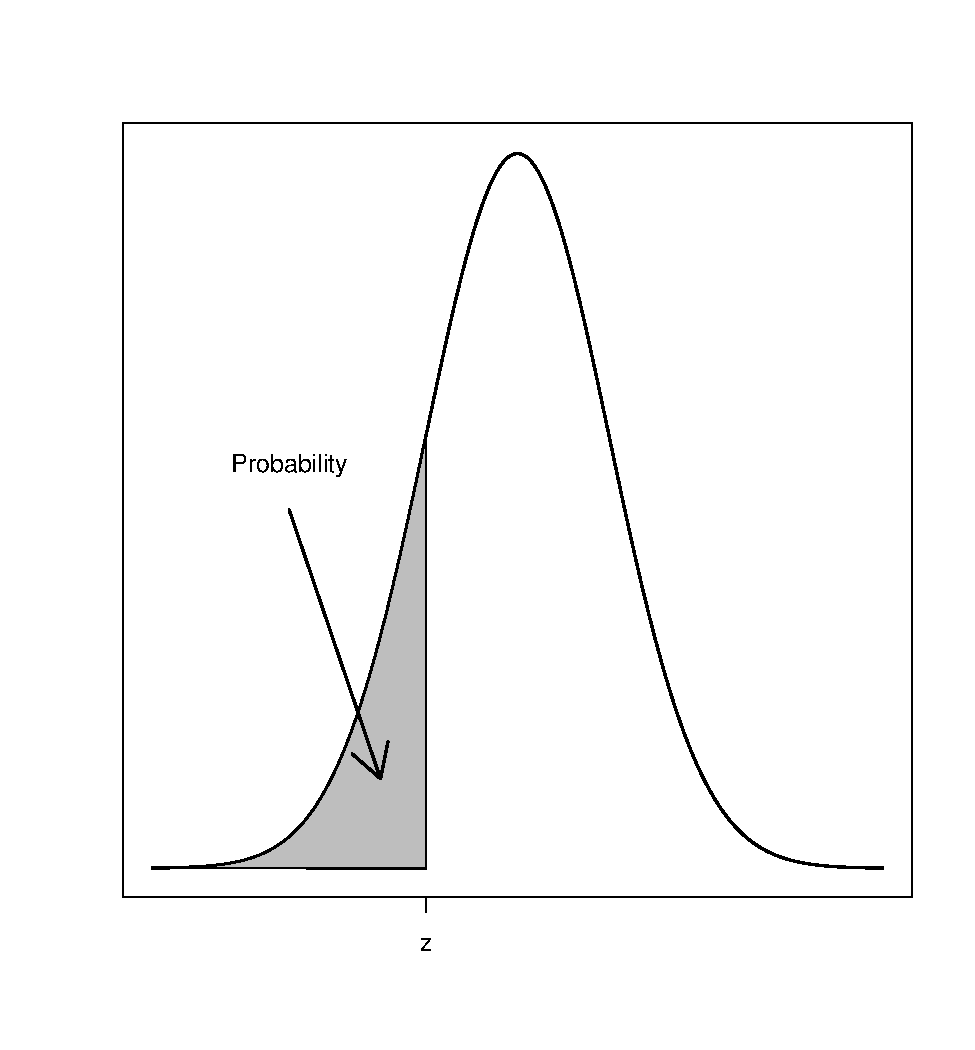
\includegraphics{_main_files/figure-latex/unnamed-chunk-35-1.pdf}

Click for table of standard normal probabilities

Table entry for \(z\) is the probability lying below \(z\).

\(z\)

0.00

0.01

0.02

0.03

0.04

0.05

0.06

0.07

0.08

0.09

-3.4

0.0003

0.0003

0.0003

0.0003

0.0003

0.0003

0.0003

0.0003

0.0003

0.0002

-3.3

0.0005

0.0005

0.0005

0.0004

0.0004

0.0004

0.0004

0.0004

0.0004

0.0003

-3.2

0.0007

0.0007

0.0006

0.0006

0.0006

0.0006

0.0006

0.0005

0.0005

0.0005

-3.1

0.0010

0.0009

0.0009

0.0009

0.0008

0.0008

0.0008

0.0008

0.0007

0.0007

-3.0

0.0013

0.0013

0.0013

0.0012

0.0012

0.0011

0.0011

0.0011

0.0010

0.0010

-2.9

0.0019

0.0018

0.0018

0.0017

0.0016

0.0016

0.0015

0.0015

0.0014

0.0014

-2.8

0.0026

0.0025

0.0024

0.0023

0.0023

0.0022

0.0021

0.0021

0.0020

0.0019

-2.7

0.0035

0.0034

0.0033

0.0032

0.0031

0.0030

0.0029

0.0028

0.0027

0.0026

-2.6

0.0047

0.0045

0.0044

0.0043

0.0041

0.0040

0.0039

0.0038

0.0037

0.0036

-2.5

0.0062

0.0060

0.0059

0.0057

0.0055

0.0054

0.0052

0.0051

0.0049

0.0048

-2.4

0.0082

0.0080

0.0078

0.0075

0.0073

0.0071

0.0069

0.0068

0.0066

0.0064

-2.3

0.0107

0.0104

0.0102

0.0099

0.0096

0.0094

0.0091

0.0089

0.0087

0.0084

-2.2

0.0139

0.0136

0.0132

0.0129

0.0125

0.0122

0.0119

0.0116

0.0113

0.0110

-2.1

0.0179

0.0174

0.017

0.0166

0.0162

0.0158

0.0154

0.0150

0.0146

0.0143

-2.0

0.0228

0.0222

0.0217

0.0212

0.0207

0.0202

0.0197

0.0192

0.0188

0.0183

-1.9

0.0287

0.0281

0.0274

0.0268

0.0262

0.0256

0.0250

0.0244

0.0239

0.0233

-1.8

0.0359

0.0351

0.0344

0.0336

0.0329

0.0322

0.0314

0.0307

0.0301

0.0294

-1.7

0.0446

0.0436

0.0427

0.0418

0.0409

0.0401

0.0392

0.0384

0.0375

0.0367

-1.6

0.0548

0.0537

0.0526

0.0516

0.0505

0.0495

0.0485

0.0475

0.0465

0.0455

-1.5

0.0668

0.0655

0.0643

0.0630

0.0618

0.0606

0.0594

0.0582

0.0571

0.0559

-1.4

0.0808

0.0793

0.0778

0.0764

0.0749

0.0735

0.0721

0.0708

0.0694

0.0681

-1.3

0.0968

0.0951

0.0934

0.0918

0.0901

0.0885

0.0869

0.0853

0.0838

0.0823

-1.2

0.1151

0.1131

0.1112

0.1093

0.1075

0.1056

0.1038

0.1020

0.1003

0.0985

-1.1

0.1357

0.1335

0.1314

0.1292

0.1271

0.1251

0.1230

0.1210

0.1190

0.1170

-1.0

0.1587

0.1562

0.1539

0.1515

0.1492

0.1469

0.1446

0.1423

0.1401

0.1379

-0.9

0.1841

0.1814

0.1788

0.1762

0.1736

0.1711

0.1685

0.1660

0.1635

0.1611

-0.8

0.2119

0.2090

0.2061

0.2033

0.2005

0.1977

0.1949

0.1922

0.1894

0.1867

-0.7

0.2420

0.2389

0.2358

0.2327

0.2296

0.2266

0.2236

0.2206

0.2177

0.2148

-0.6

0.2743

0.2709

0.2676

0.2643

0.2611

0.2578

0.2546

0.2514

0.2483

0.2451

-0.5

0.3085

0.305

0.3015

0.2981

0.2946

0.2912

0.2877

0.2843

0.281

0.2776

-0.4

0.3446

0.3409

0.3372

0.3336

0.3300

0.3264

0.3228

0.3192

0.3156

0.3121

-0.3

0.3821

0.3783

0.3745

0.3707

0.3669

0.3632

0.3594

0.3557

0.3520

0.3483

-0.2

0.4207

0.4168

0.4129

0.4090

0.4052

0.4013

0.3974

0.3936

0.3897

0.3859

-0.1

0.4602

0.4562

0.4522

0.4483

0.4443

0.4404

0.4364

0.4325

0.4286

0.4247

0.0

0.5000

0.4960

0.4920

0.4880

0.4840

0.4801

0.4761

0.4721

0.4681

0.4641

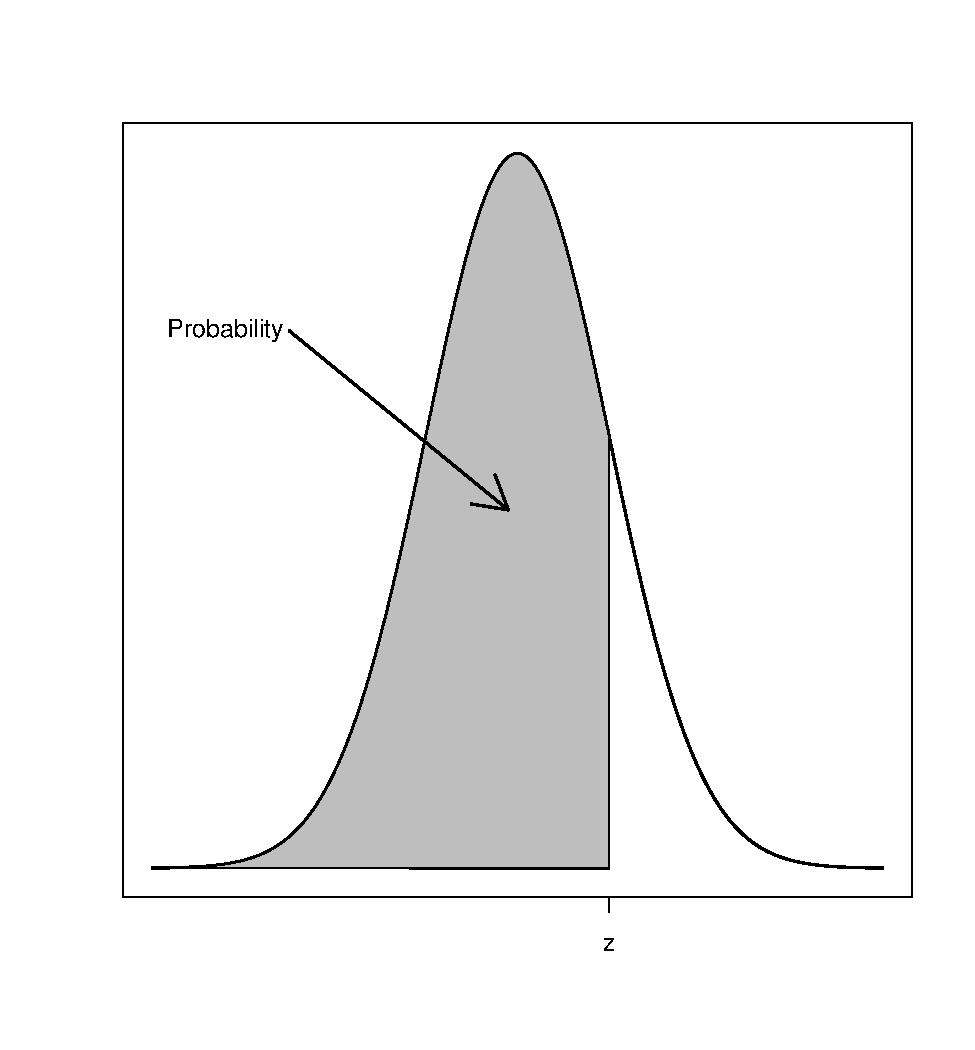
\includegraphics{_main_files/figure-latex/unnamed-chunk-36-1.pdf}

Click for table of standard normal probabilities (continued)

Table entry for \(z\) is the probability lying below \(z\).

\(z\)

0.00

0.01

0.02

0.03

0.04

0.05

0.06

0.07

0.08

0.09

0.0

0.5000

0.5040

0.5080

0.5120

0.5160

0.5199

0.5239

0.5279

0.5319

0.5359

0.1

0.5398

0.5438

0.5478

0.5517

0.5557

0.5596

0.5636

0.5675

0.5714

0.5753

0.2

0.5793

0.5832

0.5871

0.5910

0.5948

0.5987

0.6026

0.6064

0.6103

0.6141

0.3

0.6179

0.6217

0.6255

0.6293

0.6331

0.6368

0.6406

0.6443

0.6480

0.6517

0.4

0.6554

0.6591

0.6628

0.6664

0.6700

0.6736

0.6772

0.6808

0.6844

0.6879

0.5

0.6915

0.6950

0.6985

0.7019

0.7054

0.7088

0.7123

0.7157

0.7190

0.7224

0.6

0.7257

0.7291

0.7324

0.7357

0.7389

0.7422

0.7454

0.7486

0.7517

0.7549

0.7

0.7580

0.7611

0.7642

0.7673

0.7704

0.7734

0.7764

0.7794

0.7823

0.7852

0.8

0.7881

0.7910

0.7939

0.7967

0.7995

0.8023

0.8051

0.8078

0.8106

0.8133

0.9

0.8159

0.8186

0.8212

0.8238

0.8264

0.8289

0.8315

0.8340

0.8365

0.8389

1.0

0.8413

0.8438

0.8461

0.8485

0.8508

0.8531

0.8554

0.8577

0.8599

0.8621

1.1

0.8643

0.8665

0.8686

0.8708

0.8729

0.8749

0.8770

0.8790

0.8810

0.8830

1.2

0.8849

0.8869

0.8888

0.8907

0.8925

0.8944

0.8962

0.8980

0.8997

0.9015

1.3

0.9032

0.9049

0.9066

0.9082

0.9099

0.9115

0.9131

0.9147

0.9162

0.9177

1.4

0.9192

0.9207

0.9222

0.9236

0.9251

0.9265

0.9279

0.9292

0.9306

0.9319

1.5

0.9332

0.9345

0.9357

0.9370

0.9382

0.9394

0.9406

0.9418

0.9429

0.9441

1.6

0.9452

0.9463

0.9474

0.9484

0.9495

0.9505

0.9515

0.9525

0.9535

0.9545

1.7

0.9554

0.9564

0.9573

0.9582

0.9591

0.9599

0.9608

0.9616

0.9625

0.9633

1.8

0.9641

0.9649

0.9656

0.9664

0.9671

0.9678

0.9686

0.9693

0.9699

0.9706

1.9

0.9713

0.9719

0.9726

0.9732

0.9738

0.9744

0.9750

0.9756

0.9761

0.9767

2.0

0.9772

0.9778

0.9783

0.9788

0.9793

0.9798

0.9803

0.9808

0.9812

0.9817

2.1

0.9821

0.9826

0.9830

0.9834

0.9838

0.9842

0.9846

0.9850

0.9854

0.9857

2.2

0.9861

0.9864

0.9868

0.9871

0.9875

0.9878

0.9881

0.9884

0.9887

0.9890

2.3

0.9893

0.9896

0.9898

0.9901

0.9904

0.9906

0.9909

0.9911

0.9913

0.9916

2.4

0.9918

0.9920

0.9922

0.9925

0.9927

0.9929

0.9931

0.9932

0.9934

0.9936

2.5

0.9938

0.9940

0.9941

0.9943

0.9945

0.9946

0.9948

0.9949

0.9951

0.9952

2.6

0.9953

0.9955

0.9956

0.9957

0.9959

0.9960

0.9961

0.9962

0.9963

0.9964

2.7

0.9965

0.9966

0.9967

0.9968

0.9969

0.9970

0.9971

0.9972

0.9973

0.9974

2.8

0.9974

0.9975

0.9976

0.9977

0.9977

0.9978

0.9979

0.9979

0.9980

0.9981

2.9

0.9981

0.9982

0.9982

0.9983

0.9984

0.9984

0.9985

0.9985

0.9986

0.9986

3.0

0.9987

0.9987

0.9987

0.9988

0.9988

0.9989

0.9989

0.9989

0.9990

0.9990

3.1

0.9990

0.9991

0.9991

0.9991

0.9992

0.9992

0.9992

0.9992

0.9993

0.9993

3.2

0.9993

0.9993

0.9994

0.9994

0.9994

0.9994

0.9994

0.9995

0.9995

0.9995

3.3

0.9995

0.9995

0.9995

0.9996

0.9996

0.9996

0.9996

0.9996

0.9996

0.9997

3.4

0.9997

0.9997

0.9997

0.9997

0.9997

0.9997

0.9997

0.9997

0.9997

0.9998

\hypertarget{table-b-t-distribution-critical-values}{%
\section{\texorpdfstring{Table B \(t\) distribution critical values}{Table B t distribution critical values}}\label{table-b-t-distribution-critical-values}}

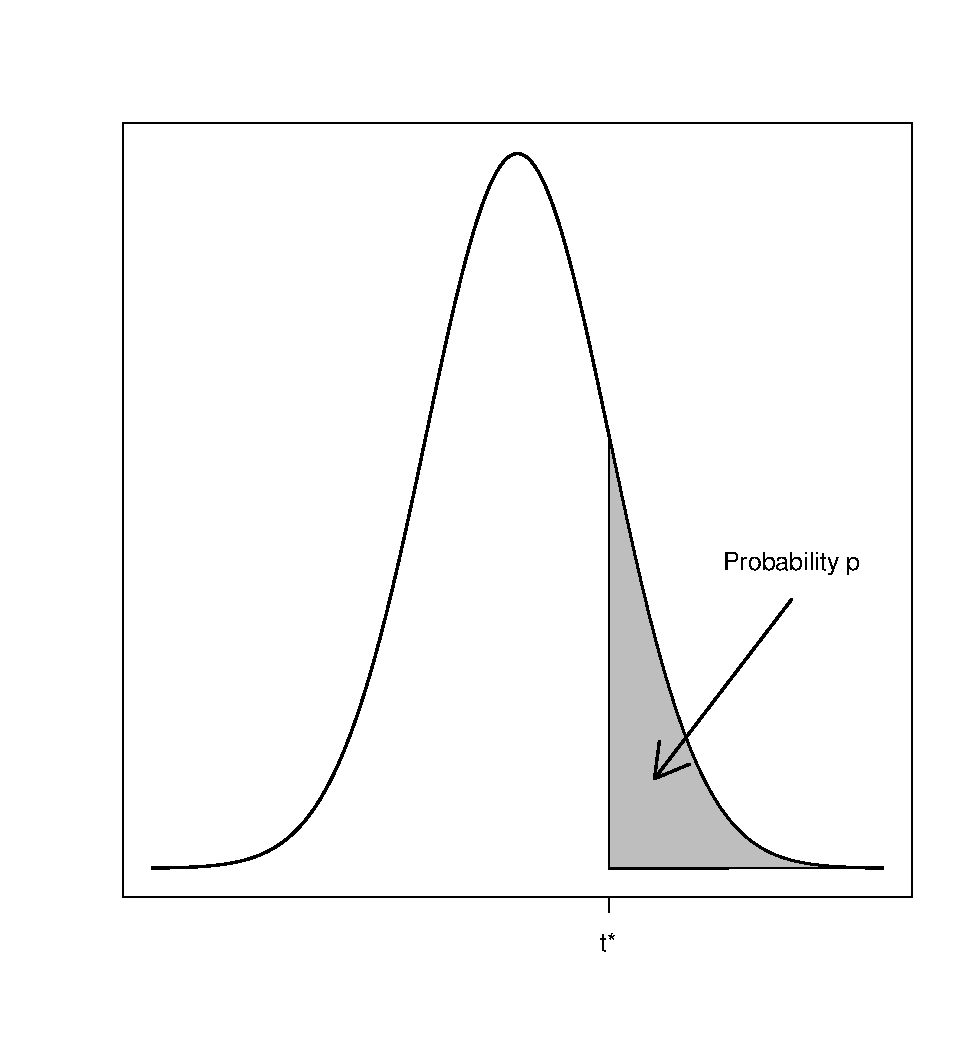
\includegraphics{_main_files/figure-latex/unnamed-chunk-37-1.pdf}

Click here for table of \(t\) distribution critical values

Table entry for \(p\) and \(C\) is the point \(t*\) with probability \(p\) lying above it and probability \(C\) lying between \(-t*\) and \(t*\).

df

Tail Probability \(p\)

0.25

0.20

0.15

0.10

0.05

0.025

0.02

0.01

0.005

0.0025

0.001

0.0005

1

1.000

1.376

1.963

3.078

6.314

12.71

15.89

31.82

63.66

127.3

318.3

636.6

2

0.816

1.061

1.386

1.886

2.920

4.303

4.849

6.965

9.925

14.09

22.33

31.60

3

0.765

0.978

1.250

1.638

2.353

3.182

3.482

4.541

5.841

7.453

10.21

12.92

4

0.741

0.941

1.190

1.533

2.132

2.776

2.999

3.747

4.604

5.598

7.173

8.610

5

0.727

0.920

1.156

1.476

2.015

2.571

2.757

3.365

4.032

4.773

5.893

6.869

6

0.718

0.906

1.134

1.440

1.943

2.447

2.612

3.143

3.707

4.317

5.208

5.959

7

0.711

0.896

1.119

1.415

1.895

2.365

2.517

2.998

3.499

4.029

4.785

5.408

8

0.706

0.889

1.108

1.397

1.860

2.306

2.449

2.896

3.355

3.833

4.501

5.041

9

0.703

0.883

1.100

1.383

1.833

2.262

2.398

2.821

3.250

3.690

4.297

4.781

10

0.700

0.879

1.093

1.372

1.812

2.228

2.359

2.764

3.169

3.581

4.144

4.587

11

0.697

0.876

1.088

1.363

1.796

2.201

2.328

2.718

3.106

3.497

4.025

4.437

12

0.695

0.873

1.083

1.356

1.782

2.179

2.303

2.681

3.055

3.428

3.930

4.318

13

0.694

0.870

1.079

1.350

1.771

2.160

2.282

2.650

3.012

3.372

3.852

4.221

14

0.692

0.868

1.076

1.345

1.761

2.145

2.264

2.624

2.977

3.326

3.787

4.140

15

0.691

0.866

1.074

1.341

1.753

2.131

2.249

2.602

2.947

3.286

3.733

4.073

16

0.690

0.865

1.071

1.337

1.746

2.120

2.235

2.583

2.921

3.252

3.686

4.015

17

0.689

0.863

1.069

1.333

1.740

2.110

2.224

2.567

2.898

3.222

3.646

3.965

18

0.688

0.862

1.067

1.330

1.734

2.101

2.214

2.552

2.878

3.197

3.610

3.922

19

0.688

0.861

1.066

1.328

1.729

2.093

2.205

2.539

2.861

3.174

3.579

3.883

20

0.687

0.860

1.064

1.325

1.725

2.086

2.197

2.528

2.845

3.153

3.552

3.850

21

0.686

0.859

1.063

1.323

1.721

2.080

2.189

2.518

2.831

3.135

3.527

3.819

22

0.686

0.858

1.061

1.321

1.717

2.074

2.183

2.508

2.819

3.119

3.505

3.792

23

0.685

0.858

1.060

1.319

1.714

2.069

2.177

2.500

2.807

3.104

3.485

3.768

24

0.685

0.857

1.059

1.318

1.711

2.064

2.172

2.492

2.797

3.091

3.467

3.745

25

0.684

0.856

1.058

1.316

1.708

2.060

2.167

2.485

2.787

3.078

3.450

3.725

26

0.684

0.856

1.058

1.315

1.706

2.056

2.162

2.479

2.779

3.067

3.435

3.707

27

0.684

0.855

1.057

1.314

1.703

2.052

2.158

2.473

2.771

3.057

3.421

3.690

28

0.683

0.855

1.056

1.313

1.701

2.048

2.154

2.467

2.763

3.047

3.408

3.674

29

0.683

0.854

1.055

1.311

1.699

2.045

2.150

2.462

2.756

3.038

3.396

3.659

30

0.683

0.854

1.055

1.310

1.697

2.042

2.147

2.457

2.750

3.030

3.385

3.646

40

0.681

0.851

1.050

1.303

1.684

2.021

2.123

2.423

2.704

2.971

3.307

3.551

50

0.679

0.849

1.047

1.299

1.676

2.009

2.109

2.403

2.678

2.937

3.261

3.496

60

0.679

0.848

1.045

1.296

1.671

2.000

2.099

2.390

2.660

2.915

3.232

3.460

80

0.678

0.846

1.043

1.292

1.664

1.990

2.088

2.374

2.639

2.887

3.195

3.416

100

0.677

0.845

1.042

1.290

1.660

1.984

2.081

2.364

2.626

2.871

3.174

3.390

1000

0.675

0.842

1.037

1.282

1.646

1.962

2.056

2.330

2.581

2.813

3.098

3.300

\(\infty\)

0.674

0.842

1.036

1.282

1.645

1.960

2.054

2.326

2.576

2.807

3.090

3.291

50\%

60\%

70\%

80\%

90\%

95\%

96\%

98\%

99\%

99.50\%

99.8

99.99\%

Confidence Level \(C\)

\end{document}
